\chapter{Markdown}
[转]\url{http://elegantlatex.org/2014/06/11/markdown-first-start}

在 ubuntu 下可以用 ReText 编辑器。
在 Mac OS/Windows 下可以用 typora 编辑器。

\section{简介}
Markdown 的目标是实现「易读易写」。

可读性,无论如何,都是最重要的。一份使用 Markdown 格式撰写的文件应该可以直接以纯文本发布,并且看起来不会像是由许多标签或是格式指令所构成。Markdown 语法受到一些既有 text-to-HTML 格式的影响,包括 Setext、atx、Textile、reStructuredText、Grutatext 和 EtText,而最大灵感来源其实是纯文本电子邮件的格式。

总之, Markdown 的语法全由一些符号所组成,这些符号经过精挑细选,其作用一目了然。比如:在文字两旁加上星号,看起来就像强调。Markdown 的列表看起来,嗯,就是列表。Markdown 的区块引用看起来就真的像是引用一段文字,就像你曾在电子邮件中见过的那样。


\section{段落文字编写}
\subsection{空格与断行}
\begin{itemize}
\item 单个空格与多个空格效果是一样的(单个空格)
\item 单个回车视为空格,多个回车视为断行
\end{itemize}
这点跟\LaTeX 输入是一样的。


\subsection{斜体与加粗}
斜体只需在斜体文字左右加星号(*)或下划线(\_)即可,而粗体需要加双星号(**)或双下划线(\_\_)。注意: 星号或者下划线应该与斜体或者加粗字体相连,不能有空格。

示例代码:
\begin{verbatim}
*斜体示例 Italic words and sentences*

_斜体示例 Italic words and sentences_

**黑体示例 Bold Face samples**

__黑体示例 Bold Face samples__
\end{verbatim}


\subsection{引用文字}
引文使用 > 开头。


\subsection{标题}
Markdown 标题等级有六级,从一级标题到六级标题分别由 \# 到 \#\#\#\#\#\# 表示。

示例代码:
\begin{verbatim}
# 一级标题示例
## 二级标题示例
### 三级标题示例
...
###### 六级标题,最末等级标题
\end{verbatim}


\subsection{列表}
列表有两类,分别为有序列表和无序列表,有序列表使用1、2、3 … 引导,无序列表使用星号(*)、加号(+)或者减号(-)引导,且三者的效果是一样的(同一等级的话)。并且列表之间是可以嵌套的。

示例代码 (无序列表):
\begin{verbatim}
* Candy.
    + Candy.
    + Gum.
    + Booze.
* Gum.
    - Candy.
    - Gum.
    - Booze.
* Booze.
\end{verbatim}

示例代码 (有序列表):
\begin{verbatim}
1. Red
    1. Red
    2. Green
    3. Blue
2. Green
    + Candy.
    + Gum.
    + Booze.
3. Blue
\end{verbatim}



\section{超链接}
Markdown 支持两种形式的链接语法:行内和参考两种形式,两种都是使用括号把文字转成链接。

\subsection{行内语法}
示例代码:

\verb|This is an [example link with title](http://example.com/ "标题 Title").|

说明:行内语法用到了方括号和圆括号,方括号表示链接在网页中的显示效果,而圆括号内为链接地址,使用双引号可以加入链接标题,这个标题是指当我们鼠标停留在链接时,网页上浮动显示的文字,链接标题是 可选项,比如:

\verb|This is an [example link without title](http://example.com/).|


\subsection{参考语法}
参考形式的链接让你可以为链接定一个名称,之后你可以在文件的其他地方(建议放在文末)定义该链接的内容。

示例代码:
\begin{verbatim}
ElegantLaTeX 的站点链接为 [ElegantLaTeX][1],其中部分内容来源于 [TeX Stack Exchange][2],
作为更全面的一个站点,我们推荐 [LaTeX Studio][3].

[1]: http://elegantlatex.org/ "ElegantLaTeX"
[2]: http://tex.stackexchange.com/ "TeX.Stack.Exchange"
[3]: http://www.latexstudio.net/ "LaTeX Studio"
\end{verbatim}


\section{插图}
图片的语法和链接很像,区别在开头加一个惊叹号!。同样,图片插入也有两种方式,一种是行内,一种是参考引用。


\subsection{行内语法}
示例代码:
\begin{verbatim}
我们 ElegantLaTeX 的图标是 ![ElegantLaTeX Logo](http://elegantlatex.qiniudn.com/
wp-content/uploads/2014/05/logo-e1400431970427.png "ElegantLaTeX Logo")
\end{verbatim}


\subsection{参考语法}
参考语法的格式和超链接的几乎一致,比如我们要显示百度的 Logo 使用下面的代码:

示例代码:
\begin{verbatim}
百度的图标为 ![百度 Logo][4]。

[4]: http://www.baidu.com/img/baidu_sylogo1.gif "百度"
\end{verbatim}


\section{代码显示}
\subsection{行内代码}
Markdown 中代码显示比较简单,行内代码使用反引号` 来标记代码区段。

示例代码:
\begin{verbatim}
在 LaTeX 中调用宏包的命令为`\usepackage{pkg.name}`,其中 `pkg.name` 为宏包名。
\end{verbatim}


\subsection{行间代码}
行间代码只要每行都缩进 4 个空格或是一个 tab 就可以了。
\begin{verbatim}
 C++ code

    public class Blog
    {
        public int Id { get; set; }
        public string Subject { get; set; }
    }
\end{verbatim}


\section{$\backslash$的作用}
反斜杠 $\backslash$  可以显示 \verb|*_+-`| 等在 Markdown 中有特殊意义的字符。


















\chapter{Fortran}
\begin{comment}
\begin{itemize}
\item 语句并行写\\
 \verb| a=1.0  ;  b=2.0|,即在同一行语句间要加分号(不同行语句间不用)。

\item 语句续行写\\
F90中一行为132列,允许有39个续行。在语句行最后加上续行符“\&”号。如果字符串被打断,跨2行以上,则在续行的开始位置也要加\&号。如:
\begin{verbatim}
inter : : v( 7 , 7 ) , &
         v1( 7 , 7 ) 
和
v1 = reshape( [ 1.0d0 , 0.0d0 , 0.0d0 , 0.0d0 , 0.0d0 , 0.0d0 , 0.0d0 , &
           &   0.0d0 , 0.0d0 , 0.0d0 , 0.0d0 , 0.0d0 , 0.0d0 , 0.0d0 , &
           &   0.0d0 , 0.0d0 , 0.0d0 , 0.0d0 , 0.0d0 , 0.0d0 , 0.0d0 , &
           &   0.0d0 , 0.0d0 , 0.0d0 , 0.0d0 , 0.0d0 , 0.0d0 , 0.0d0 , &
           &   0.0d0 , 0.0d0 , 0.0d0 , 0.0d0 , 0.0d0 , 0.0d0 , 0.0d0 , &
           &   0.0d0 , 0.0d0 , 0.0d0 , 0.0d0 , 0.0d0 , 0.0d0 , 0.0d0 , &
           &    0.0d0 , 0.0d0 , 0.0d0 , 0.0d0 , 0.0d0 , 0.0d0 , 0.0d0 ] , [ 7 , 7] , order=[2,1] )
\end{verbatim}

\item fortran数组的第一个指标是行数,第二个是列数,但在内存中存储是相反的,这个不要混淆了。

\item 矩阵运算函数 \verb|matmul(A,B)|其中\verb|A(7,7),B(7,7)|

\item nint将x转换为整数(四舍五入)。详见:FORTRAN 90标准函数 
\verb|nint(a)|,取a最接近的整数。
\end{itemize}
\end{comment}


\section{哑元}
%\url{http://blog.163.com/jey_df/blog/static/18255016120111021105343466/}
\begin{itemize}
\item intent(in) 表示这个参数是输入的;
\item intent(out) 表示参数是输出的;
\item intent(inout)表示这个参数同时用于两个方向的数据传递。
\end{itemize}

哑实结合是在两个程序单元间传递数值的主要手段,主程序中实元2.0与过程中哑元X结合,就使X有值2.0,也即把主程序中2.0的值传递给子程序中的X,该值可供子程序运算。反之,如果子程序中的变量Y在子程序执行完后有值3.0,它与实元R结合后则使调用程序单元中的实元变量R得值3.0。

在F77中,不能确切地说明哑元的目的。它们到底是用于把数据传入到过程中的,还是用于把数据传出到调用它的程序单元中的,或是两者兼而有之的,这个概念是含糊的。在F90中,为了避免当过程内部变量值变化后返回到引用的程序单元时可能造成的混淆情况,在过程的变量类型的定义中,可以对哑元指定意图说明的INTENT属性。哑元按数据传输特性可分为输入输出两用、仅用于输入和仅用于输出。其一般形式为:
\begin{itemize}
\item 在类型定义语句中:\verb|类型, INTENT(意图说明符) :: 哑元名表|,如:\verb|real*8, intent(in) :: X|;
\item 或用INTENT语句 :\verb|INTENT(意图说明符) :: 哑元名表|,如:\verb|intent(in) :: X|。
\end{itemize}
推荐使用第一种形式。意图说明符为以下字符串:
\begin{itemize}
\item IN :指明哑元仅用于向过程提供数据,过程的执行期间哑元不能被重定义或成为未定义的,相联合的实元可以是常数、变量、数组以及它们的算术表达式;

\item OUT :指明哑元用于把过程中的数据传回调用过程的程序,与之相结合的实元只允许是变量,不得为常数或算术表达式;

\item INOUT :指明哑元既可以用于向过程提供数据,也可用于向调用程序返回数据,与之相结合的实元只允许是变量。
\end{itemize}

INTENT属性不能在主程序说明语句中出现,只能在过程的哑元说明语句中使用。它是可选的,可省略。但现代特性的编程中应提倡使用INTENT属性,因为这样能增加可读性和可维护性,还能防止编程中的一些错误。因为一旦哑实结合,哑元和实元始终是同一个值,如果过程中给有属性INTENT(IN)的哑元重新赋值,也将改变调用程序单元中实元的值,而这是不应该的。这样,如在程序执行部分中误把有INTENT(IN)属性的哑元赋值时,操作系统就会提示。


\section{双冒号}
在新的语法里,很多变量类型后书写两个冒号,然后是变量名。

双冒号,表示修饰符的结束。例如:

\verb|Integer , parameter , private :: fcode( 3 , 3 )|

Integer 是变量类型,它有两个修饰符:parameter 和 private,两个冒号表示修饰符结束了,也就是说,如果有修饰符,则必须有双冒号。

语法还规定,如果定义变量时,同时对其赋予初始值,则变量默认具有 save 属性,此时相当于隐藏了 save 这个修饰符,因此也必须有双冒号。
例如:\verb|integer :: a = 0| ,实际是 \verb|integer , save :: a = 0| ,因此不能简写为:\verb|integer a=0|。

因此,也建议在所有定义语句中使用双冒号。


\section{浮点型变量声明的格式}
单精度浮点数的声明方法單(使用4个字节)
\begin{verbatim}
real(kind=4) x_float !Fortran 90
real(4) y_float            !Fortran 77
real*4 z_float             !Fortran 77
\end{verbatim}

双精度浮点数的声明方法(使用8个字节)
\begin{verbatim}
real(kind=8) x_double !Fortran 90
real(8) y_double            !Fortran
real*8 z_double             !Fortran
\end{verbatim}



\section{输入输出的格式命令}
格式命令,[]中的可省略  
\begin{itemize}
\item Aw :以w个字符宽度来输出字符串;
\item BN :定义文本框中的空位为没有东西,在输入时才需要使用;  
\item BZ :定义文本框中的空位代表0,输入时才需要使用; 
\item Dw.d: 以w个字符宽来输出指数类型的浮点数,小数部分占d个字符宽;  
\item Ew.d[Ee]:以w个字符宽度来输出指数类型的浮点数,小数部分占d个字符宽,指数部分占e个字符;  
\item ENw.d[Ee]:以指数类型来输出浮点数,工程计数法  
\item ESw.d[Ee]: 以指数类型来输出浮点数,科学计数法  
\item Fw.d:以w个字符宽来输出浮点数,小数部分占d个字符宽;  
\item Gw.d[Ee]:以w个字符宽度来输出任何种类的数据;  
\item Iw[.m]:以w个字符宽来输出整数,最少输出m个数字;  
\item Lw:以w个字符宽来输出T或F的真假值;  
\item nX:把输出的位置向右跳过n个位置;  
\item /:换行;  
\item :  :在没有更多数据时结束输出;  
\item kP:K值控制输入输出的SCALE;  
\item Tn:输出的位置移动到本行第n列;  
\item TLn:输出的位置向左相对移动n列;  
\item TRn:输出的位置向右相对移动n列;  
\item SP:在数值为正时加上“正号”;  
\item SS:取消SP;  
\item 以下Fortran 90 添加
	\begin{itemize}
	\item Bw[.m]:把整数转换成二进制来输出,输出会占w个字符宽,固定输出m个数字,m值可以不给定;  
	\item Ow[.m]:把整数转换成八进制来输出,输出会占w个字符宽,固定输出m个数字,m值可以不给定 ; 
	\item Zw[.m]:把整数转换成十六进制来输出,输出会占w个字符宽,固定输出m个数字,m值可以不给定;
	\end{itemize}
\end{itemize}




\section{整数转字符串——产生序列文件名}
整型转字符,借助FORTRAN语言的内部文件完成,即将一个字符串变量当作一个内部文件来看待。给一个实用的例子吧。

假如你有一组文件有20个,命名规律是myFile*.dat,其中*是从1到20递增的整型数,则要用循环依次打开这些文件可以这样写:
\begin{lstlisting}[language=Fortran]
program main
implicit none

character( len = 2 ) :: cTemp
integer :: k

do k = 1, 20

write( cTemp,'(i2)' ) k
open ( 1, file = 'myFile' // trim(adjustl( cTemp )) // '.dat', status = 'old' )
!...
close( 1 )

end do

end porgram main
\end{lstlisting}

这里因为k可能是一位数,也可能是两位数,所以字符串变量cTemp的长度至少要是2个字符长度,才能保证最大整数能装下。trim和adjustl是FORTRAN的标准内部函数。adjustl的作用是将字符串里的内容左对齐,空格置于右端。trim的作用是将字符串末尾(即右端)的空格删掉。这样无论你的k是一位数还是两位数,都可以保证open路径中不会出现多余的空格。// 是FORTRAN的字符串操作符,作用是将字符串连接起来。

同理,如果是字符型数字转整型或实型,方法一样,比如:
\begin{lstlisting}[language=Fortran]
character( len = 4 ) :: cTemp = '2007'
integer :: year

read( cTemp, '(i4)' ) :: year
!%%%%%%%%%%%%%%%%%%%%%%%%%%%%%%%%%%%%
  CHARACTER*3   STR  
  WRITE(STR,'(A3)')123  
  此时STR作为内部文件使用
!%%%%%%%%%%%%%%%%%%%%%%%%%%%%%%%%%%%%
Use a character string variable as an "internal file", write the file
: name you want to this string (like sprintf in C), and use the string.
: character(len=12)::fname
: integer::i
: do i=0,9999,1
: write(unit=fname,fmt="('file',i4.4,'.dat')")i ! like sprintf() in C
: open(unit=10,file=fname)
: ...
: close(unit=10)
: end do
编制有限元程序时,经常要用到序列文件名,如:
file001.txt, file002.txt, ...

贴出源程序,供各位参考:

文件名: NAMEGEN.F90
******************************************************************


MODULE NAMEGEN_

CONTAINS


! *****************************************************************

FUNCTION NAMEGEN (NAME, NUM, INDEX, EXT)

! *****************************************************************
!
! 程序说明:
! Generate sorted file name. Attach the number after each filename.
! The conversion of integer value into character is used.
!
! INPUT:
! NAME filename;
! NUM indicate the maximum file number
!                                          used, e.g. 
! "0000","00000";
! INDEX the number of this file;
! EXT extension of the file;
! EXAMPLE:
! NAME='FILE'
! NUM='0000'
! INDEX=18
! EXT='TXT'
! Returned name is: FILE0018.TXT
!
! Xin Zhao, 2002-2-12
! *****************************************************************

CHARACTER*108 NAMEGEN,NA,NUM1
CHARACTER*(*) NAME,EXT,NUM
INTEGER*4 INDEX,LENGTH1,LENGTH2
WRITE(NA,'(I4)') INDEX
NA=ADJUSTL (NA)
LENGTH1=LEN_TRIM(NA)
LENGTH2=LEN_TRIM(NUM)
NUM1=NUM(1:(LENGTH2-LENGTH1))//NA
NAMEGEN=TRIM(NAME)//TRIM(NUM1)//'.'//TRIM(EXT)
END FUNCTION

END MODULE
\end{lstlisting}


\section{Fortran格式输出——不换行与换行}
\verb|write (file_number,format_spec,advance='no')| 这样写就不会自动换行,而格式中如果加入`\verb|\|'则是换行和\verb|\n|一样。

实例:

原来的:
\begin{lstlisting}[language=Fortran]
	open( unit = 10, file = "real_rho.ods" )
	write( 10, 100 )  t/fs ,   real( y0( 1, 1, 1 ) ) , &
                                     &  real( y0( 1, 2, 2 ) ) , &
                                     &  real( y0( 1, 3, 3 ) ) , &
                                     &  real( y0( 1, 4, 4 ) ) , &
                                     &  real( y0( 1, 5, 5 ) ) , &
                                     &  real( y0( 1, 6, 6 ) ) , &
                                     &  real( y0( 1, 7, 7 ) )
       100 format( 8(f14.7 , ',') )
	200 format( 8(A8 , ',' ) )
\end{lstlisting}

改:
\begin{lstlisting}[language=Fortran]
open(unit = 10, file = "real_rho.ods" )
write(10, 100, advance='no')  t/fs
do j = 1, nsite-1
	write(10, 100, advance='no')  real( y0(1,j,j) ) 
enddo
write(10, 100) real(y0(1,nsite,nsite))
100 format( 3(f14.7 , ',') )
200 format( 1(A8 , ',' ) )
\end{lstlisting}
新改的程序适应性更强,不用手动修改输出。



\section{getarg、iargc、trim的用法}
getarg用法:\verb|call getarg(NUMBER,VALUE)|其中NUMBER是获取第几个参数,VALUE是相应的值。
iargc用法:\verb|n=iargc()|,返回命令行中参数的数量。

getarg是用来返回你输入的命令行参数的。

\verb|call getarg(n,buffer)|

其中$n$是命令序号, buffer是相应的命令行参数。运行程序本身的命令是0号,跟在它后面的参数是1,2。。。号。

比如,你写这样一个小程序:
\begin{lstlisting}[language=Fortran]
character*80 buff
call getarg(0,buff)
write(*,*) buff
call getarg(1, buff)
write(*,*) buff
call getarg(2, buff )
write (*,*) buff
end
\end{lstlisting}
然后编译它,比如把这个可执行程序命名为mypro,然后键入命令如下

Linux系统,键入

./mypro   ar1 ar2

可以看到结果是

./mypro

ar1

ar2

Windows下,则键入

mypro ar1 ar2

可看到结果是

mypro

ar1

ar2

可见,用命令行方式,程序执行命令本身是第0个参数,后面跟的第1,2。。个参量则可以用相应的getarg来获得。利用这个getarg,你可以在外部输入命令时控制程序中的一些东西。



\section{huge}













\chapter{C\&C++}
\section{Linux下的开源编译器}
C与C++用的是不同的编译器

C++ 要用g++ hello.cpp -o hello

C  可以用gcc hello.cpp -o hello

\#define 和 const 与区别:const 进行数据类型检查,而define只是简单的替换

src是source的缩写,这里是源文件的意思。“source”本身是“源”的意思。


\section{数组的下标}
同时用不同语言编程的话,很容易被各自特点搞晕。C\&C++的数组下标索引默认是从0开始的,而 Fortran 默认是从1开始的。最要命的是C\&C++的数组下标越界还不报错。例如给两个数组赋值。
\begin{verbatim}
double G[3]={0.0};
double P[3]={0.0};
G[1] = 1.7835;
G[2] = 0.666;
G[3] = 0.3615;
P[1] = 16.94475;
P[2] = 40.78275;
P[3] = 6.07425;
\end{verbatim}
这里数组越界了,但编译运行时不会报错。两个数组在内存中是连续储存的。在内存中其真实值为:
\begin{verbatim}
G[0] = 0.0;
G[1] = 1.7835;
G[2] = 0.666; 
P[0] = 0.3615; // 本应赋值给G数组第3个数的,现在却赋值给P数组的第一个数了。
P[1] = 16.94475;
P[2] = 40.78275;
\end{verbatim}

严格来说,C\&C++语言中没有多维数组,通常所说的多维数组其实是数组的数组。谨记这一点,对理解和使用多维数组大有益处。






\chapter{C}
\section{static关键字解析}
\url{http://blog.csdn.net/wu_zf/article/details/7068326}

static 声明的变量在C语言中有两方面的特征:

\begin{itemize}
\item 变量会被放在程序的全局存储区中,这样可以在下一次调用的时候还可以保持原来的赋值。这一点是它与堆栈变量和堆变量的区别。

\item 变量用static告知编译器,自己仅仅在变量的作用范围内可见。这一点是它与全局变量的区别。
\end{itemize}

有时希望函数中的局部变量的值在函数调用结束后不消失而保留原值,即其占用的存储单元不释放,在下一次函数调用时,该变量已有值,就是上一次函数调用结束时的值。这是就应该指定该局部变量为“局部静态变量”,用static加以说明。

在C语言中,关键字static有三个明显的作用:
\begin{itemize}
\item 在函数体,一个被声明为静态的变量在这一函数被调用过程中维持其值不变。
\item 在模块内(但在函数体外),一个被声明为静态的变量可以被模块内所用函数访问,但不能被模块外其它函数访问。它是一个本地的全局变量。
\item 在模块内,一个被声明为静态的函数只可被这一模块内的其它函数调用。那就是,这个函数被限制在声明它的模块的本地范围内使用。
\end{itemize}

static 全局变量与普通全局变量的区别:

在定义变量时,全局变量之前再冠以 static 就构成了静态的全局变量。全局变量本身就是静态存储方式,静态全局变量当然也是静态存储方式。两者在存储方式上并无不同。两者的区别在于非静态全局变量的作用域是整个源程序,当一个源程序由多个源文件组成时,非静态的全局变量在各源文件中都是有效的。而静态全局变量则限制了其作用域,即只在定义该变量的源文件内有效,在同一源程序的其他源文件中不能使用。由于静态全局变量的作用域局限域于一个源文件内,只能为该源文件内的函数使用,因此可以避免其他源文件 使用该变量。把普通全局变量改变为静态全局变量是改变了他的作用域,限制了他的使用范围。

static 局部变量和普通局部变量的区别:

普通局部变量所在的函数每次被调用都会被重新定义并分配存储空间,而 static 局部变量不会,他的值始终保存着。static 局部变量只被初始化一次,下一次使用时依旧是上一次的值。

static 函数与普通函数的区别:

static 函数(即静态函数,在函数定义时加上了static 关键字)与普通函数作用域不同,他仅存在于文本文件中。只在当前源文件中使用的函数应该说明为内部函数(即加上static关键字)。内部函数应该在当前 源文件中声明和定义。对于可在当前源文件以外的函数,应该在一个头文件中说明,要使用这个函数的源文件要包含这个头文件。另:程序的普通全局变量存在于堆 栈中,全局变量、static 局部变量存在于静态存储区中。



\section{文件操作}
\url{http://www.cnblogs.com/whiteyun/archive/2009/08/08/1541822.html}
\subsection{文件的基本概念}
\subsubsection{文件}
所谓“文件”是指一组相关数据的有序集合。 这个数据集有一个名称,叫做文件名。文件通常是驻留在外部介质(如磁盘等)上的,在使用时才调入内存中来。从不同的角度可对文件作不同的分类。

从用户的角度看,文件可分为普通文件和设备文件两种。

普通文件是指驻留在磁盘或其它外部介质上的一个有序数据集,可以是源文件、目标文件、可执行程序; 也可以是一组待输入处理的原始数据,或者是一组输出的结果。对于源文件、目标文件、 可执行程序可以称作程序文件,对输入输出数据可称作数据文件。

设备文件是指与主机相联的各种外部设备,如显示器、打印机、键盘等。在操作系统中,把外部设备也看作是一个文件来进行管理,把它们的输入、输出等同于对磁盘文件的读和写。 通常把显示器定义为标准输出文件,一般情况下在屏幕上显示有关信息就是向标准输出文件输出。如前面经常使用的printf,putchar 函数就是这类输出。键盘通常被指定标准的输入文件, 从键盘上输入就意味着从标准输入文件上输入数据。scanf,getchar函数就属于这类输入。

从文件编码的方式来看,文件可分为ASCII码文件和二进制码文件两种。

ASCII文件也称为文本文件,这种文件在磁盘中存放时每个字符对应一个字节,用于存放对应的ASCII码。例如,数5678的存储形式为:

\begin{center}
\begin{tabular}{lcccc}
ASC码:&00110101&00110110&00110111&00111000\\
                &$\downarrow$&$\downarrow$&$\downarrow$&$\downarrow$\\
十进制码:&5&6&7&8 
\end{tabular}
\end{center}
共占用4个字节。ASCII码文件可在屏幕上按字符显示, 例如源程序文件就是ASCII文件。 由于是按字符显示,因此能读懂文件内容。

二进制文件是按二进制的编码方式来存放文件的。 例如, 数5678的存储形式为: 00010110 00101110只占二个字节。二进制文件虽然也可在屏幕上显示,但其内容无法读懂。C系统在处理这些文件时,并不区分类型,都看成是字符流,按字节进行处理。输入输出字符流的开始和结束只由程序控制而不受物理符号(如回车符)的控制。 因此也把这种文件称作“流式文件”。在C语言中,文件操作都是由库函数来完成的。



\subsubsection{文件指针}
在C语言中用一个指针变量指向一个文件, 这个指针称为文件指针。通过文件指针就可对它所指的文件进行各种操作。定义说明文件指针的一般形式为: FILE *指针变量标识符; 其中FILE应为大写,它实际上是由系统定义的一个结构,该结构中含有文件名、文件状态和文件当前位置等信息。 在编写源程序时不必关心FILE结构的细节。

例如:FILE *fp;表示fp是指向FILE结构的指针变量,通过fp 即可找存放某个文件信息的结构变量,然后按结构变量提供的信息找到该文件,实施对文件的操作。习惯上也笼统地把fp称为指向一个文件的指针。



\subsubsection{文件的打开与关闭}
文件在进行读写操作之前要先打开,使用完毕要关闭。所谓打开文件,实际上是建立文件的各种有关信息,并使文件指针指向该文件,以便进行其它操作。关闭文件则断开指针与文件之间的联系,也就禁止再对该文件进行操作。



\subsection{fopen函数}
fopen函数用来打开一个文件,其调用的一般形式为:
\begin{center}
文件指针名= fopen(文件名,使用文件方式) 
\end{center}
其中,“文件指针名”必须是被说明为FILE 类型的指针变量,“文件名”是被打开文件的文件名。 “使用文件方式”是指文件的类型和操作要求。“文件名”是字符串常量或字符串数组。例如: 

FILE *fp;

fp=fopen("a.pdb","r");

其意义是在当前目录下打开文件a.pdb, 只允许进行“读”操作,并使fp指向该文件。





\chapter{C++}
\section{文件包含处理\#include}
\subsection{文件包含的作用}
所谓“文件包含”处理是指一个源文件可以将另外一个源文件的全部内容包含进来,即将另外的文件包含到本文件之中。C++提供了\#include命令用来实现“文件包含”的操作。如在file1.cpp中有以下\#include命令:\#include ″file2.cpp″,它的作用见下图。

%\inlcudegraphics{pictures/wjbh.png}

“文件包含”命令是很有用的,它可以节省程序设计人员的重复劳动。

\#include命令的应用很广泛,绝大多数C++程序中都包括\#include命令。现在,库函数的开发者把这些信息写在一个文件中,用户只需将该文件“包含”进来即可(如调用数学函数的,应包含cmath文件—),这就大大简化了程序,写一行\#include命令的作用相当于写几十行、几百行甚至更多行的内容。这种常用在文件头部的被包含的文件称为“标题文件”或“头部文件”。

头文件一般包含以下几类内容:
\begin{itemize}
\item 对类型的声明;
\item 函数声明;
\item 内置(inline)函数的定义;
\item 宏定义, 用\#define定义的符号常量和用const声明的常变量;
\item 全局变量定义;
\item 外部变量声明,如entern int a;
\item 还可以根据需要包含其他头文件。
\end{itemize}

不同的头文件包括以上不同的信息,提供给程序设计者使用,这样,程序设计者不需自己重复书写这些信息,只需用一行\#include命令就把这些信息包含到本文件了,大大地提高了编程效率。由于有了\#include命令,就把不同的文件组合在一起,形成一个文件。因此说,头文件是源文件之间的接口。


\subsection{include命令的两种形式}
在\#include命令中,文件名除了可以用尖括号括起来以外,还可以用双撇号括起来。\#include命令的一般形式为:\#include <文件名>或 \#include ″文件名″。如:\#include <iostream>或 \#include ″iostream″都是合法的。二者的区别是: 用尖括号时,系统到系统目录中寻找要包含的文件,如果找不到,编译系统就给出出错信息。

有时被包含的文件不一定在系统目录中,这时应该用双撇号形式,在双撇号中指出文件路径和文件名。如果在双撇号中没有给出绝对路径,如\#include ″file2.c″则默认指用户当前目录中的文件。系统先在用户当前目录中寻找要包含的文件,若找不到,再按标准方式查找。如果程序中要包含的是用户自己编写的文件,宜用双撇号形式。

对于系统提供的头文件,既可以用尖括号形式,也可以用双撇号形式,都能找到被包含的文件,但显然用尖括号形式更直截了当,效率更高。


\section{关于C++标准库}
在C++编译系统中,提供了许多系统函数和宏定义,而对函数的声明则分别存放在不同的头文件中。如果要调用某一个函数,就必须用\#include命令将有关的头文件包含进来。C++的库除了保留C的大部分系统函数和宏定义外,还增加了预定义的模板和类。但是不同C++库的内容不完全相同,由各C++编译系统自行决定。不久前推出的C++标准将库的建设也纳入标准,规范化了C++标准库,以便使C++程序能够在不同的C++平台上工作,便于互相移植。新的C++标准库中的头文件一般不再包括后缀.h,例如:  \#include <string>

但为了使大批已有的C程序能继续使用,许多C++编译系统保留了C的头文件,即提供两种不同的头文件,由程序设计者选用。如:

    \#include <iostream.h>  //C形式的头文件

    \#include <iostream>  //C++形式的头文件

效果基本上是一样的。建议尽量用符合C++标准的形式,即在包含C++头文件时一般不用后缀。如果用户自己编写头文件,可以用.h为后缀。




\chapter{LabVIEW}
\section{注意事项}
\begin{itemize}
\item 多使用快捷键;
\item 尽量不要将输入和输出控件显示为图标形式,可以大大增大操作空间;
\item 经常添加说明信息;
\item 注意VI的图标和连线版处理;
\item 即时帮助很重要,最好一直打开;
\item 编程要避免功能混乱。
\end{itemize}



\section{快捷键}
\begin{itemize}
\item Ctrl+E: 前后面板切换;
\item Ctrl+S: 保存;
\item Ctrl+Z: 撤销;
\item Ctrl+R: 运行;
\item Ctrl+H: 即时帮助,很重要;
\item Ctrl+B: 删掉悬空的线;
\item Shift+右键:切换鼠标状态;
\item 空格: 快速切换鼠标状态
\end{itemize}


\section{基本特性}
\begin{figure}[htbp]
\centering
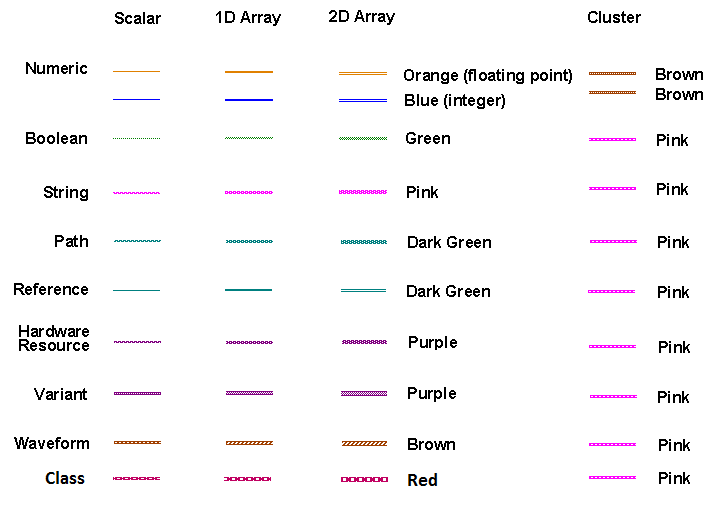
\includegraphics[width=0.8\textwidth]{pictures/Wire_Colors.png}
%\caption{The population of FMO with sink}\label{fig:1} 
\end{figure}

\begin{figure}[htbp]
\centering
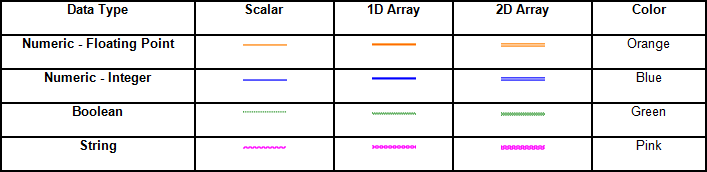
\includegraphics[width=0.8\textwidth]{pictures/wire_types.png}
%\caption{The population of FMO with sink}\label{fig:1} 
\end{figure}

\subsection{属性节点}
\subsection{事件}

\subsection{子Vi}
\begin{itemize}
\item 连线状态可以查看子Vi端口名称。
\end{itemize}



\section{用户界面设计}
界面好坏的最基本指标:
\begin{itemize}
\item 是否完成了交互功能
\item 是否可以简单直观地输入或获取信息
\item 界面的美观度
\end{itemize}

使用 Labview 开发一个项目的步骤:
\begin{itemize}
\item 收集需求; 
\item 设计;
\item 编码;
\item 测试;
\item 发布及维护
\end{itemize}

建议:先做用户界面设计,在做程序设计

理由:先设计程序结构,再设计界面,难免会朝着最可能简化编码工作方向去做。但是这样的界面往往不是最方便用户使用的界面。

另一方面,使用比较老的文本语言编程,设计用户界面时通常在草稿纸上画出原型。LabVIEW有独特的优势,可视化编程做的非常方便。有大量现成的控件,控件属性更改非常方便。因此,用户可以通过拖拽的方式,直接用LabVIEW来设计界面原型。

好的用户界面共有的特点:
\begin{itemize}
\item 一致性
\item 使用恰当的数据类型和控件类型;
\item 控件的分类排布合理、简洁
\end{itemize}

一致性:
让用户迅速接受并且方便的操作一个程序界面,最关键的一点就是让这个界面保存高度的一致性。

一致性包含以下多个方面的一致:
\begin{itemize}
\item 程序内部的一致性;\\
由于应用领域、面向的客户群体的不同,不同的软件可以有自己独特的风格。不论一个程序采用哪种风格,它内部不同界面,同一面板上的不同控件等,它们的风格应当保持一致。一个软件采用统一的风格,才会让用户有一种协调的感觉。
\item 与约定俗成的习惯保持一致;\\
很多设计或操作方法,已经被大家广为接受。它们也许不见得美观或优化,但是一旦习惯养成了,就很难被改变了。
\item 与真实事物保持一致;\\
有很多程序是对现实世界的模拟或模仿,这样的程序若希望便于被用户接受,最好是尽量与现实世界保持一致。LabVIEW编写的程序大多是测量、控制等有关,在这些领域,原本也存在着一些相关的仪器或设备。因此软件的界面可以借鉴这些仪器的外观。
\item 建立并遵循界面规范。\\
使界面保持一致性的最好办法就是在设计开发时遵循一定的规范。这个规范可以由公司内部定义,也可以遵循现有的行业规范。对于开发Windows系统风格的程序,可以遵循微软定义的界面规范。对于一般的LabVIEW程序,可以遵循LabVIEW程序开发规范。
\end{itemize}

界面元素的关联:

当一个界面上的元素比较多,找到自己想要的信息就要花上一小点时间。用户常常是一眼就看到了一个与自己想要的信息有一点关联的某个元素,他这时候会期望这个元素就有一定的提示信息,帮他加速找到自己想要的东西。因此,我们要在界面上,告诉用户哪些元素是相关的,或不相关的。

有很多手段可以把界面的元素之间的关联现实给用户,比如通过元素的排布、边框、空白、颜色、字体等等方式。我们总是在相关内容的附近去找想要的信息,所以逻辑上相关的控件或项目,应当在屏幕空间上相对临近。
单纯的把条目排在一起还是不利于用户查看。可以把它们按功能分成几个不同的区域,比如保存文件与 Project的操作在功能上相对独立一些,就可以用分隔线,帮它们的项目划分开。对于面板上的控件,功能相关的几个控件可以通过被边框围住、使用分割线、采用不同的间隙等等方法,让用户直观的感觉到他们在功能上的紧密关联。

帮助和反馈信息:

用户界面要照顾到那些不熟悉它的用户。为了方便用户了解界面的使用方法,需要给用户提供足够的帮助信息。对于 LabVIEW, 给用户提供提示主要通过以下几个手段:用户手册、在线帮助窗口、提示条、利用控件的标题、选项文字、直接把帮助文字写在界面上。不论何时,都应该尽量使用有意义的控件名称。

用户界面设计的限制:

目的:保障程序的可靠性

手段:限制用户的输入数据和操作
\begin{itemize}
\item 限制数据的输入;
\item 防止用户的误操作。
\end{itemize}



\section{调用DLL动态链接库}
参考:阮奇桢 《我和LabVIEW——一个NI工程师的十年编程经验》,北京航空航天大学出版社。感觉他写的这部分内容前后背景交代的很清楚,看起来舒服。

常用的计算机语言各有其特色,也有其不足。LabVIEW虽然功能强大,但编程时也时常会发现它缺少某些所需的功能,而这些功能也许恰恰已经有其他编程语言的DLL、ActiveX组件等提供。在这种情况下,最高效的方法莫不如让LabVIEW调用这些模块,直接利用其他语言或者操作系统已经实现的功能。


\subsection{DLL}
Dynamcis Linkable Library, DLL,动态链接库。从字母上理解,它是一种“程序库”。库内存放的是可供应用程序使用的函数、变量等。

“动态”是与“静态”相对应而来的。这里的动态和静态是指链接库中代码与使用它们的应用程序之间的链接方式。如果采用静态链接库,在生成应用程序时,库中的函数等都会被直接放入最终生成的可执行文件中;而使用动态链接库时,库中的函数等不会放到可执行文件中去,而是仍然保留在DLL文件内。当程序被运行时,再链接到动态链接库中的函数和变量等内容。

静态库的局限性比较大,C 语言编写的静态库只能在C 语言中使用,LabVIEW无法调用。而动态链接库则可以在多种编程语言中通用,即使用某一种语言编写出来的DLL可以在另一种语言编写的程序中使用。例如,使用C语言编写的DLL可以在LabVIEW中使用,反之亦可。

动态链接库的加载方式又分“动态”与“静态”两种。这里的动态和静态是指应用程序运行时,动态链接库代码被载入内存的方式。常用的方式是静态加载,指动态链接库在应用程序启动时随应用程序一起被载入内存。而动态加载方式是指,应用程序启动时并不载入动态链接库,只有在使用到动态链接库中某个函数时,才把动态链接库载入内存。

DLL最大的优势在于代表共享,只要某一功能以 DLL的形式提供出来了,其他的应用程序就可以直接使用这一功能,而不必再实现一份相同的代码了。DLL的使用非常普遍,比如 Windows 操作系统提供给应用程序调用的功能,就是以 DLL 的形式公布出来的。LabVIEW中若需使用某个系统功能,如读/写注册表等,即可通过调用 Windows 提供的 DLL 函数来完成。Windows 提供的这些完成系统功能的函数也被称为 Windows API(Application Programming Interface)。在常用的几个系统 DLL 中, kernel32.dll 提供了内存管理和进程调度相关的函数,user32.dll 中的函数则主要用于控制用户界面,gdi32.dll中的函数则负责图形方法的操作。在32位操作系统中,这些 Windows API 的 DLL 都被保存在 system32 目录下。
%
很多硬件设备的驱动程序也往往是以DLL方式提供的。此外,在互联网上还可以找到各种各样的 DLL。如果需要解析某种文件、使用某些常用的算法等,都可以先去互联网上搜索一下,是否有相关的DLL 库可供直接使用。

在LabVIEW中,经常会遇到需要使用DLL的情况,比如在程序中使用到某个以DLL方式提供的第三方驱动程序或算法;再比如,在一个大项目的开发中,出于效率和开发人员喜好等因素的考虑,可能使用C++语言实现软件的运算部分,并把这些功能构建在DLL文件中,再使用 LabVIEW 编写程序的界面部分,并通过调用编写好的 DLL 来调用运算部分的功能。


\subsection{CLN和CIN节点}
在LabVIEW中,通过“互连接口$\rightarrow$库与可执行程序$\rightarrow$调用库函数” 节点来调用 DLL 中的函数。调用库函数节点常简称为 CLN 节点,是英文 Call Library Function Node 的缩写。在同一函数选板上,它旁边的一个节点是“代码接口”(Code Interface Node),简称 CIN节点。
在CLN节点出现以前,LabVIEW只能通过CIN节点调用C 语言编写的函数。现在有了CLN,可以不再考虑使用CIN了。
CIN节点不能调用动态链接库中的函数,只能调用按照特定方式编译出来的程序代码。稍有差错,程序就无法正常运行。CIN所调用的程序模块不通用,而且限制颇多,CLN节点出现之后,就很少有人再使用CIN节点了。


\subsection{LabVIEW调用DLL中的函数以及手动配置CLN节点}
这部分在参考书中写的非常详细。这里简单说下。一个CLN节点被拖到程序框图上后,需要进行对其配置才能使用。双击CLN节点,则弹出其配置对话框,该对话框有4个选项卡,如下图所示
\begin{figure}[htbp]
\centering
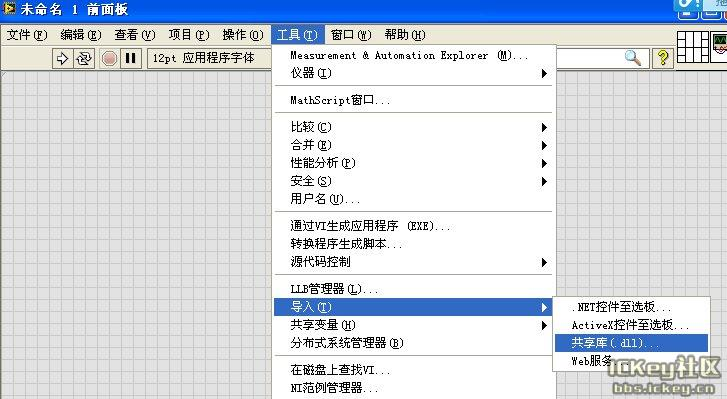
\includegraphics[width=0.9\textwidth]{pictures/1.png}
%\caption{The population of FMO with sink}\label{fig:1} 
\end{figure}
\begin{itemize}
\item 第一个选项卡是被调用函数的信息,主要有
\begin{itemize}
\item “库名或路径”列表框。用于填写DLL文件名和DLL的全路径。 在系统路径下的DLL,直接输入文件名即可,否则需要全路径。
\item “在程序框图中指定路径”选项。若没有勾选,则是LabVIEW静态调用了这个DLL;若勾选,则是动态调用。具体说明参见参考书。
\item “函数名”列表框。用于输入需要调用的DLL中的函数。如果选用静态加载方式,并已输入了正确的DLL文件全路径,这里会列出DLL中所有允许被外部调用的函数,用户只要在下拉列表框中选取一个即可。
\item “线程”选项。用于选择被调用的DLL函数在何线程内运行。 CLN节点的线程选项只有两项:“在UI线程中运行”和“在任一线程中运行”。在程序框图上直接就可以看出一个CLN节点选用的是什么线程。如果是“在UI线程中运行”,则节点颜色是比较深的桔黄色;如果是“在任一线程中运行”,则节点是比较淡的黄色。详细说明见参考书。
\item “调用规范”。用于指明被调用函数的参数压栈规范。Windows API一般使用 stdcall,标准C的库函数大多使用C call。
\end{itemize}
\item 第二个选项卡是配置参数选项卡。使用CLN节点,最困难部分就是把函数参数的数据类型映射为相应的LaVIEW中的数据类型。这也是最关键的。
\item 第三个选项卡是设置回掉函数选项卡。可以使用这些回调函数在特定的情形下完成初始化、清理资源等工作。如果为 Reserve 选择了一个回调函数,那么当一个新的线程开始调用这个 DLL 时,这个回调函数首先被调用。可以利用这个函数为新线程使用到的数据做初始化工作。如果一个线程使用了这个 DLL,在线程结束时,它会去调用 Unreserve 中指定的回调函数。Abort 中指定的函数用在 VI 非正常结束时被调用。比如按 Abort 按钮让一个 VI 停止,而不是让它运行完。这里的几个回调函数必须要由 DLL 的开发者按照特定的格式实现。它的原型就是 Prototype for these procedures 中列出的那个。如果你使用的 DLL 不是专为 LabVIEW 设计的,一般不会包含这样的回调函数。
\item 第四个是错误处理方式选项卡。这上面说明写得已经很详细了。
\end{itemize}


%\subsubsection{数据类型参数的设置}



\subsection{把DLL中的函数包装成子VI}
在LabVIEW中调用DLL的函数,最大的困难在于把函数参数的数据类型映射为相应的LabVIEW中的数据类型。在手工设置CLN节点前,可以优先考虑使用导入共享库工具,以自动生成配置CLN节点。这个工具在“工具$\rightarrow$导入$\rightarrow$共享库”菜单项中,专门用于把DLL中的函数包装成VI,生成的每个VI中最主要的部分就是一个CLN节点;它能够自动设置函数的参数。有了这个工具,用户就不再需要费脑筋去考虑数据类型匹配的问题了。

这个工具可能无法直接处理一些非常特殊的数据类型(如字符串数组)和函数(如回调函数),但在大多数情况下,都能够把DLL中的函数包装成可以正确运行的VI。如果有现成的DLL打算在LabVIEW中使用,首先应该考虑用这个工具,把DLL中所有的函数都包装成VI,再使用起来,就方便多了。

如果DLL是C++编写的,并且使用了C++的类作为接口,这样的DLL是没办法在LabVIEW中直接调用的。CLN节点只能调用符合标准C语言函数接口的DLL。若项目中必须使用某个C++ DLL,则可以在其上再用C语言写一个C接口DLL,作为它和LabVIEW之间的中间层。LabVIEW调用这个中间层DLL提供的函数,中间层函数再调用C++接口的DLL函数。



\subsubsection{应用举例}
Labview是一个图形化软件库,不但支持NI官网硬件,还支持众多第三方硬件,这些硬件提供的驱动基本上是DLL的方式,需要在labview里面调用。其实,labview也可以支持自制MCU硬件。只要能提供相应的DLL就行,甚至,如果能在labview和IDE开发环境之间建立接口,一个labview子VI,就可以实现在labview运行状态下,配合MCU仿真器,实现  图形化程序到MCU的下载,脱离了C代码的编写,开发更加快速很方便!

     今天为大家分享一个深度调用DLL的方法,为什么是深度调用DLL。因为,调用的不是DLL本身。而是由DLL生成的子VI函数。下面重点分享如何将DLL生成可以被labveiw调用的子VI。


一、要会编写DLL

     动态链接库英文为DLL,是Dynamic Link Library 的缩写形式,DLL是一个包含可由多个程序同时使用的代码和数据的库。编写DLL文件需要有VC++功底。比如平时经常开发MCU软件,积累了很多C驱动代码,如果能够按照规范,就可以生称DLL文件。
     
     二、要有相应的DLL.H文件
     
     编写了DLL文件外,还要有H文件才行。通常开发数据采集卡的厂家只会提供DLL文件本身,而不会提供编写DLL文件用的C代码和H文件。所以,那些数据采集卡只能采用直接调用DLL的方式。而自制硬件中,C代码和H文件是自己编写,所以,可以很容易实现DLL转labview的子VI。


三、应用实例讲解:

     因为一个MCU内容太多,短时间内实现也不现实。就采用一个开源厂家的例子来实现。
CH375是国内厂家江苏沁恒(\url{www.wch.cn})生产的一个USB芯片,支持HOST主机方式和SLAVE设备方式。速度可以实现全速方式,在一些总线设备和USB数据采集设备上采用很多。厂家开源了一CH375DLL.DLL和一个CH375DLL.H文件。下面分享一下过程:


\newpage
1、打开labview界面,建立一个空VI。在【工具】选项中,选择导入—共享库(dll),如图:
\begin{figure}[htbp]
\centering
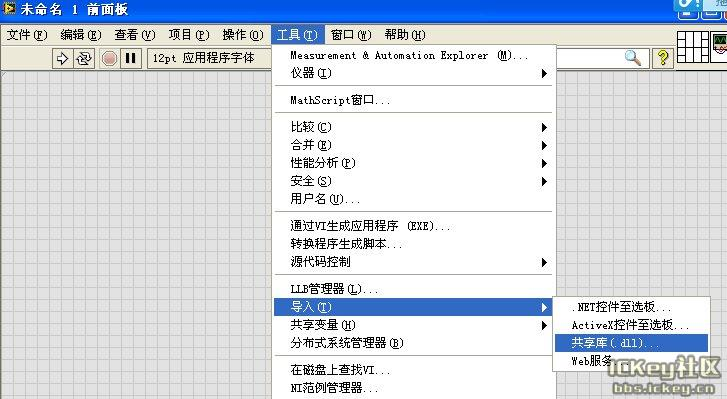
\includegraphics[width=0.9\textwidth]{pictures/1.jpg}
%\caption{The population of FMO with sink}\label{fig:1} 
\end{figure}

2、在出现的界面中,为共享库创建新Vi,进入下一步:
\begin{figure}[h!]
\centering
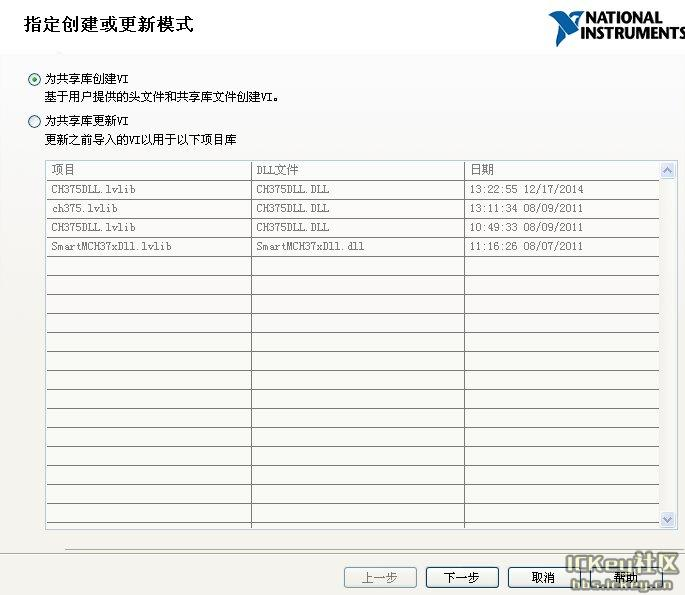
\includegraphics[width=0.9\textwidth]{pictures/2.jpg}
%\caption{The population of FMO with sink}\label{fig:1} 
\end{figure}

\newpage
3、选择共享库及头文件,这里把CH375DLL.DLL和CH375DLL.H文件载入:
\begin{figure}[h!]
\centering
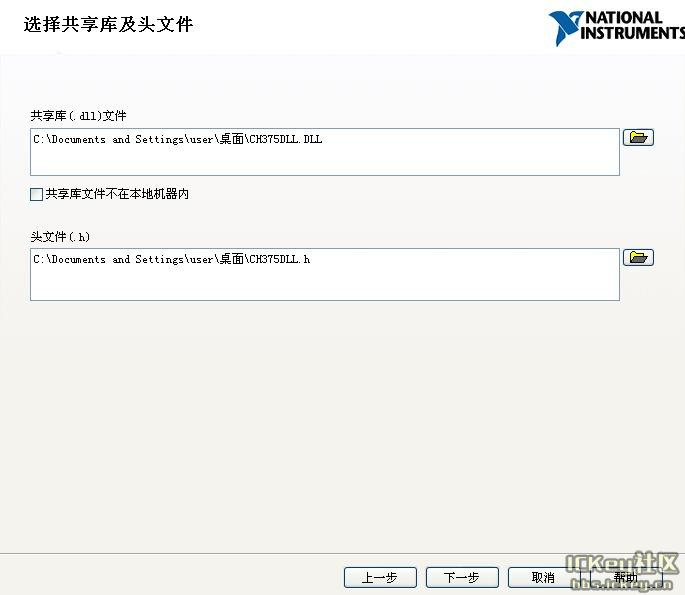
\includegraphics[width=0.75\textwidth]{pictures/3.jpg}
%\caption{The population of FMO with sink}\label{fig:1} 
\end{figure}

4、配置包路径和宏定义命令,这里空着不填,进入下一步:
\begin{figure}[h!]
\centering
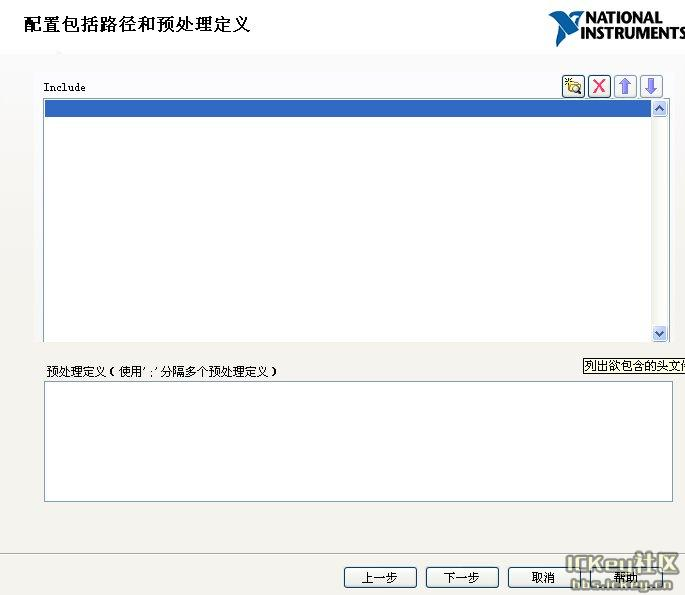
\includegraphics[width=0.75\textwidth]{pictures/4.jpg}
%\caption{The population of FMO with sink}\label{fig:1} 
\end{figure}

5、全部勾选DLL库里面的函数定义文件,下一步:
\begin{figure}[h!]
\centering
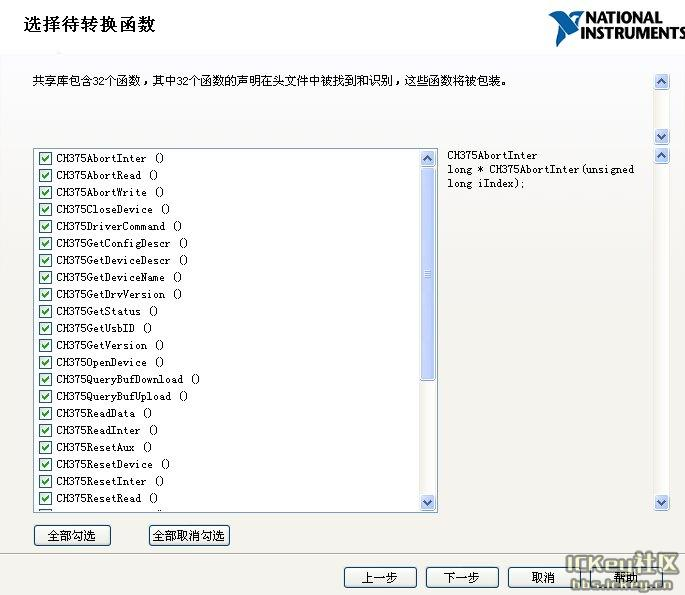
\includegraphics[width=0.75\textwidth]{pictures/5.jpg}
%\caption{The population of FMO with sink}\label{fig:1} 
\end{figure}

 6、配置好生成的VI库的路径和名称:
\begin{figure}[h!]
\centering
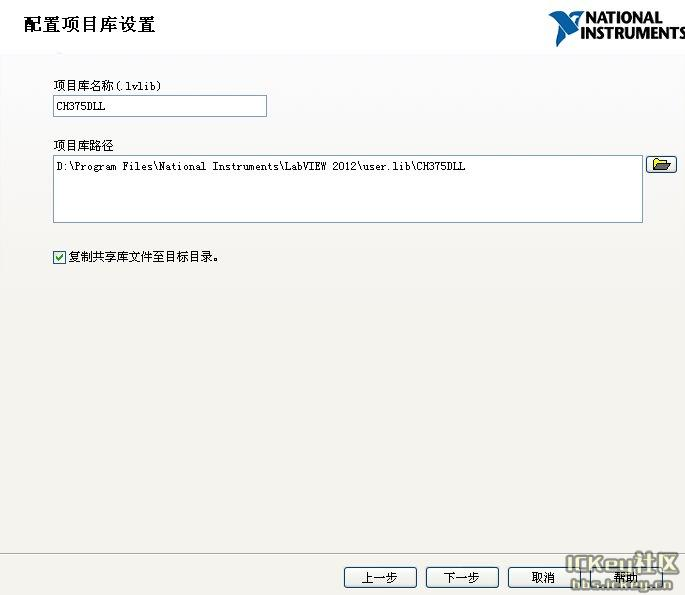
\includegraphics[width=0.75\textwidth]{pictures/6.jpg}
%\caption{The population of FMO with sink}\label{fig:1} 
\end{figure}

7、选择错误处理方式,这里有多种方式,可以选择简易错误处理:
\begin{figure}[h!]
\centering
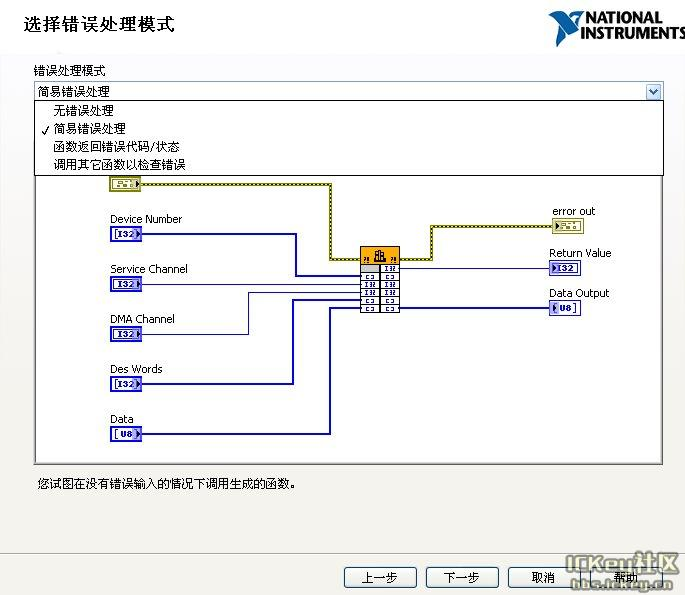
\includegraphics[width=0.75\textwidth]{pictures/7.jpg}
%\caption{The population of FMO with sink}\label{fig:1} 
\end{figure}

8、配置VI和控件,这里和DLL一样设置如图:
\begin{figure}[h!]
\centering
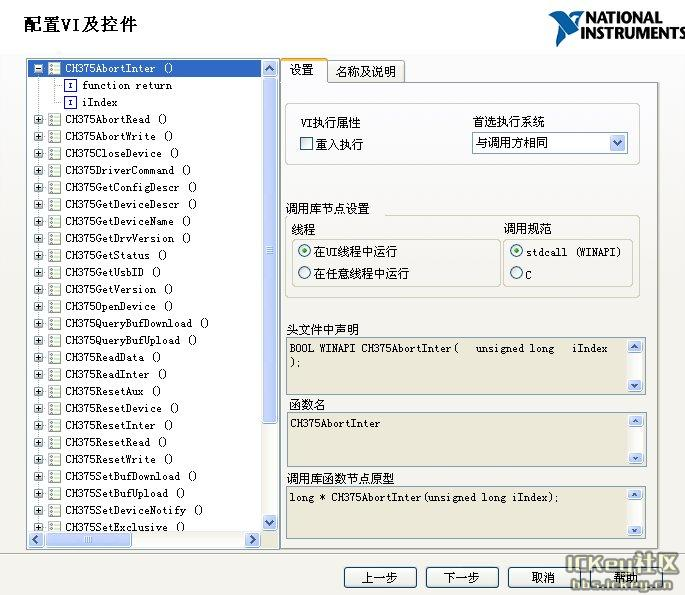
\includegraphics[width=0.75\textwidth]{pictures/8.jpg}
%\caption{The population of FMO with sink}\label{fig:1} 
\end{figure}

9、最后,是一个生成总结:
\begin{figure}[h!]
\centering
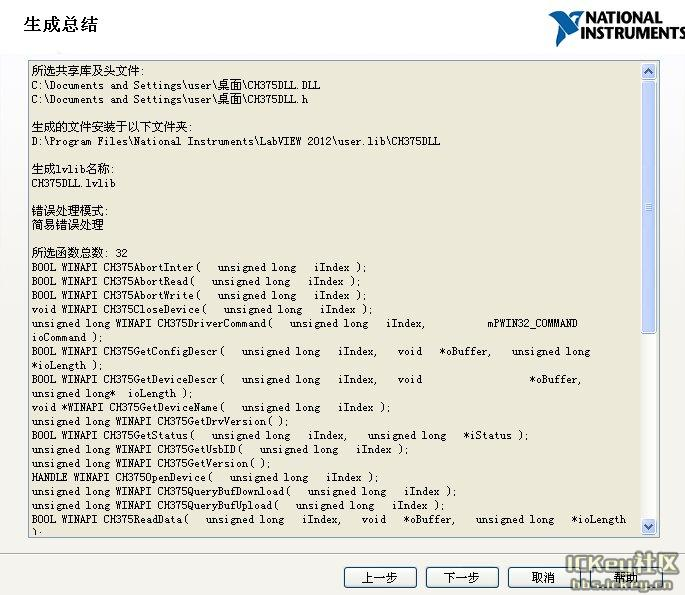
\includegraphics[width=0.75\textwidth]{pictures/9.jpg}
%\caption{The population of FMO with sink}\label{fig:1} 
\end{figure}

10、然后,点下一步就可以了:
\begin{figure}[h!]
\centering
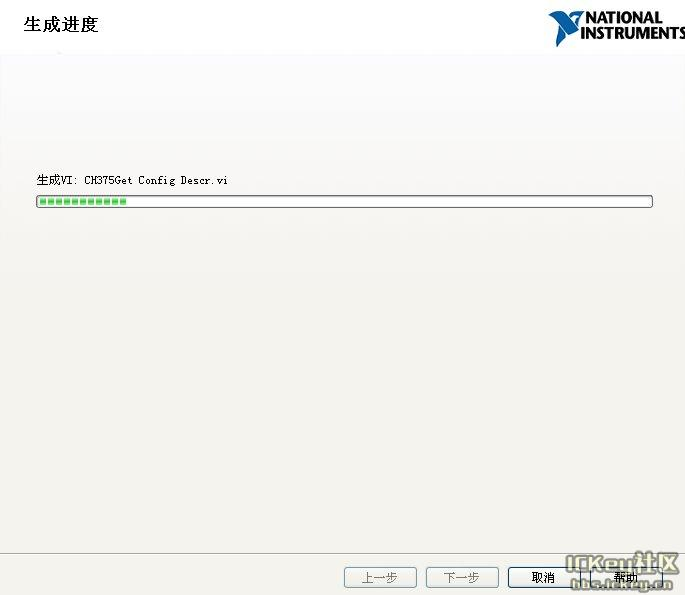
\includegraphics[width=0.75\textwidth]{pictures/10.jpg}
%\caption{The population of FMO with sink}\label{fig:1} 
\end{figure}

\begin{figure}[h!]
\centering
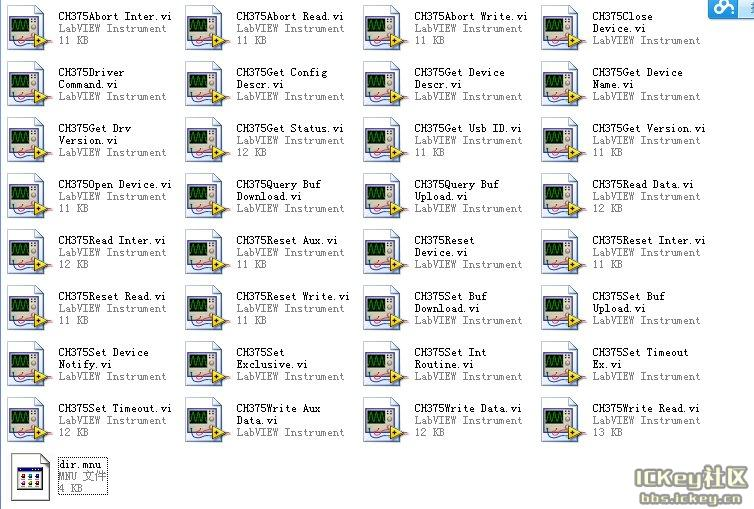
\includegraphics[width=0.75\textwidth]{pictures/11.jpg}
%\caption{The population of FMO with sink}\label{fig:1} 
\end{figure}


11、从这里调入vi,看到没,调用后,直接进行连线就可以了,不像原来那样看着眼花缭乱了。
\begin{figure}[h!]
\centering
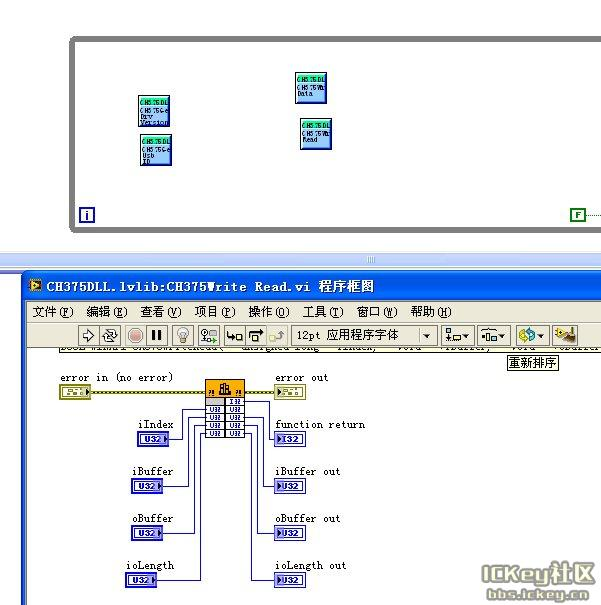
\includegraphics[width=0.75\textwidth]{pictures/13.jpg}
%\caption{The population of FMO with sink}\label{fig:1} 
\end{figure}


\subsubsection{调用DLL时遇见的问题}
在使用DLL时,最大的困难就是把函数参数的数据类型映射为相应的LabVIEW中的数据类型。LaBVIEW提示:

{\color{blue}\emph{未定义符号可能会造成函数和参数无法被识别。如要解决该问题,检查头文件并确定是否必须添加预定义符号。单击上一步按钮返回至向导的前一页并添加预定义符号(例如,“NIAPI\_stdcall \_stdcall” 或 ``NIAPIDEfined = 1'')} }

归咎原因就是头文件中哦你搞得一些类型定义不符合标准C语法,而使解析器无法获得正确的定义。DLL函数的头文件中可能使用了某个系统定义的数据类型,数据类型的定义在 windows.h中(windows.h是Windows SDK 的一个文件,VC等开发环境中常常带有 Windows SDK),要正确解析必须得到这些数据类型,也就是找到 windows.h 这个头文件,用户须把windows.h文件的全路径加在“包括路径”中。例如 Visual C++ 6.0编译环境中头文件位于安装目录下 VC98文件夹下的 Include文件中。

而“预处理定义”中,当用户需要写一些宏定义,那么就写在这个位置,如
添加如下代码:

ULONG = unsigned long; VOID = void; LONG = long; UCHAR = unsigned char; PUCHAR = unsigned char*;
PULONG = unsigned long*; WINAPI; BOOL=bool; USHORT = unsigned short; PUSHORT = unsigned short*;

这样就不会出现问题了。


\section{NI-DAQmx 数据采集}
参考书:
\begin{itemize}
\item 《LabVIEW 大学实用教程 (第三版)》 Jeffrey Travis, Jim Kring 著,乔瑞萍 等译。LabVIEW for Everyone (Graphical Programming Made Easy and Fun, Third Edition ) 第二章、第十章和第十一章。
请详细阅读相关章节。这里只记录比较重要的部分。

\item 《LabVIEW 实践教程》 Robert H. Bishop,National Instruments著,乔瑞萍 林欣 等译
\end{itemize}



\subsection{NI-DAQmx简介与安装}
(1)简介

 DAQ,Data AcQuisition,是一个术语,即数据采集,是实现测量现实世界信号如电压,并把这些信息发送到计算机用于处理、分析、储存或其他数据操作的过程。而NI-DAQmx 则是NI公司的跨平台DAQ设备驱动程序,包含了所有NI公司DAQ设备的驱动。NI-DAQmx代替了传统的NI-DAQ(以前称为“NI-DAQ”),并且在传统的NI-DAQ基础上提供了诸多改进,如:改进了状态模型、多线程驱动程序、意外情况下的健壮性、简化的同步、降低了LabVIEW框图的混乱、从简单到高级程序的平滑过渡。NI-DAQmx优于先前NI-DAQ的显著特定就是包含了DAQ Assistant以配置通道和完成测量任务。

信号的采集需要对信号有所了解,比如信号类型、一个信号的五种测量角度常见的转换器和信号调节等,这里不详细讲述,参考书中相关章节有叙述。这里需要注意的是,Nyquist-Shannnon采样定理,采样频率必须大于被采集信号最高频率的两倍。但是为了充分保持信号的形状,采样频率通常至少为信号最高频率的5$\sim$10倍。


(2)安装

NI-DAQmx是与LabVIEW单独安装的,它们版本之间的兼容性如下图所示,可以在官网查询。安装过程比较简单,跟通常软件安装过程一样,需要注意的是安装过程比较长。
\begin{figure}[h!]
\centering
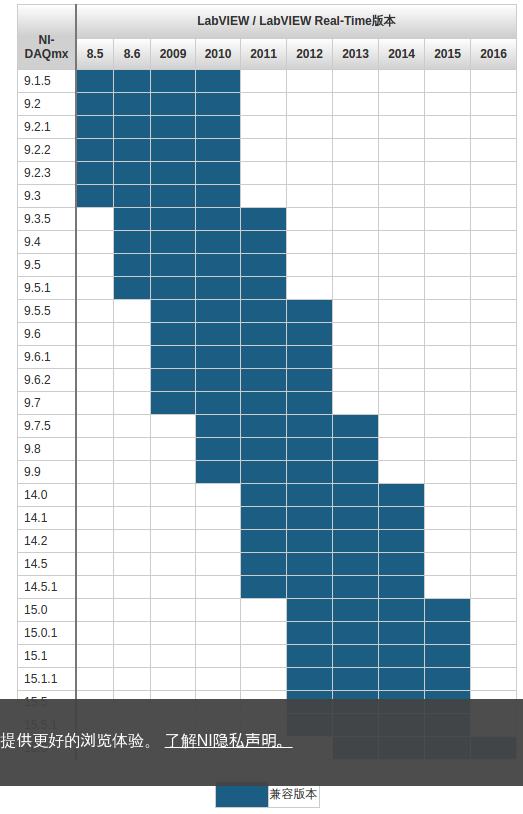
\includegraphics[width=0.5\textwidth]{pictures/ni-daqmx.png}
\caption{NI-DAQmx与LabVIEW的版本兼容性}
\end{figure}


\subsection{MAX及创建NI-DAQmx虚拟设备}
MAX,Measurement \& Automation Explorer,是在NI-DAQmx和LabVIEW之间的实用软件,目前只支持 Windows平台。它是一个Windows的软件接口,用于配置和测试硬件,可以访问NI公司的所有设备(包括DAQ,GPIB,VXI等)。换句话说,就是一个用于建立各种卡及通道配置参数的配置工具。 Windows设备管理器管理着用户系统中的所有硬件,其中包括NI公司的DAQ设备。MAX会读取设备管理器在Windows注册表中记录的信息,并为用户系统中的每个NI DAQ卡分配逻辑设备号。用户可以通过该设备号访问LabVIEW中的卡。

用户可以通过访问计算机中哦你搞得设备管理器找到数据采集设备,如 Data Acquisition Devices 中列出了安装在计算机上的所有DAQ卡。选取一个DAQ卡,选择Properties或双击该DAQ卡,可以看到一个多页面的对话框。 General 显示了与卡相关的整体信息。可以通过Resources指定该卡占用的系统资源,比如中断级、DMA以及软件可配置卡的基址。Driver指明了该DAQ卡驱动程序的版本及位置。

用户可以在NI-DAQmx7.5及新版本中利用MAX创建NI-DAQmx虚拟设备,这样用户可以建立原型系统,在进行实际数据采集前,测试数据采集应用程序。当需要实际采集时,还可以使用MAX可移植配置向导,将NI-DAQmx虚拟设备的配置输入导入到物理设备中。
创建NI-DAQmx虚拟步骤如下:
\begin{enumerate}
\item 打开MAX(Measurement \& Automation),可以点击桌面图标打开,也可以从LabVIEW打开。

\item 右击“设备和接口(Devices and Interfaces)”弹出快捷菜单并选择“新建(Create New)”。

\item 一个对话框会提示用户选择要添加的设备。选择 “仿真NI-DAQmx设备或模块化仪器(NI-DAQmx Simulated Device)” 并点击 “完成(Finish)”。

\item 在“选择设备(Choose Device)”对话框中选择需要的虚拟设备,比如 M series DAQ。

\item 选择 NI PCI-6251 并单击 OK 按钮。
\end{enumerate}


\subsection{DAQ助手}
DAQ Assistant,DAQ助手,是一个用来配置测量任务及通道的图形界面接口。DAQ助手位于 Functions>Measurement I/O>DAQmx-Data Acquisition 选项板中。将DAQ助手拖入框图中就可以将其弹出。当DAQ 助手 置入框图中时,DAQ助手对话框将会自动出现。一旦打开DAQ 助手,配置NI-DAQmx任务所需步骤与使用MAX配置NI-DAQmx任务的步骤基本一致。使用DAQ助手构建数据采集VI的通用过程如下:
\begin{itemize}
\item 打开一个新的VI。
\item 在框图中拖入DAQ 助手。
\item 出现 DAQ助手对话框帮助用户配置测量任务。
\item 配置、命名及测试NI-DAQmx任务。
\item 单击OK按钮以返回框图。
\item 编辑前面板和框图完成VI。
\end{itemize}

如果使用DAQ助手配置了DAQmx任务,则该任务就是一个本地任务,因此,它不能保存到MAX中被其他应用使用。如果想要使任务对于其他应用也可用,可是通过DAQ 助手生成NI-DAQmx Task Name控件使其保存到MAX中并在其他应用中使用。DAQmx Task Name Constant 是为了与DAQ卡进行通信而在DAQ VI中使用的一种LabVIEW数据类型。

\begin{itemize}
\item 通过右击框图中的DAQ 助手 弹出快捷菜单并在下拉菜单中选择 Convert to NI-DAQmx Task;
\item 此时会出现DAQ 助手以便重新配置任务;
\item 退出DAQ助手后,则完成转换,该DAQmx任务就存在于MAX中并且可以被其他应用使用。
\end{itemize}

如果想要在应用中使用来自MAX的DAQmx任务,则按如下步骤:
\begin{itemize}
\item 首先在 Functions>Measurement I/O>NI DAQmx-data Acquisition选项板中找到DAQmx Task Name Constant ,并拖入框图中。
\item 任务名称可以通过鼠标手形工具单击 DAQmx Task Name Constant浏览选择。
\end{itemize}



\subsection{NI-DAQmx VI}
如果说DAQ助手是数据采集的图形化配置界面,那么NI-DAQmx VI则是DAQ助手配置的底层VI。
在涉及与其他操作联动时,采用NI-DAQmx VI的形式更为可靠。
NI-DAQmx VI 是一种被称为多态VI的特殊VI,其结果是能够适应不同DAQ功能的一组核心VI,比如模拟输入、模拟输出、数字I/O等等。在LabVIEW后面板上,右键打开函数(Functions)选项板,单击“测量I/O(Measure I/O)>DAQmx 数据采集(Measurement I/O>DAQmx-data Acquisition)”访问该选项板。

Windows版的LabVIEW DAQ VI使用的是 Windows 版 32位动态链接库(DLL)形式的 NI公司标准NI-DAQ。LabVIEW安装程序将NI-DAQ DLL 安装在 Windows$\backslash$System32目录下。nidaq32.dll文件是用户使用的DAQ卡的高级接口,安装在Windows$\backslash$System32目录下。随后,nidaq32.dll文件将与Windows注册表对接以获取由MAX定义的配置参数。

NI-DAQmx VI使用非常简单,主要有如下几个步骤:
\begin{itemize}
\item 创建一个任务(或引用一个MAX DAQmx任务)。
\item 启动任务。
\item 读或写,以及根据需要重复。
\item 停止任务。
\item 清除任务。
\end{itemize}
需要注意的是:
\begin{itemize}
\item 用户不一定必须启动任务,通常读或写操作会自动启动任务。
\item 在清除任务之前不必停止任务。如果任务正在运行,清楚操作将先停止任务。
\end{itemize}




\section{EMCCD}
\subsection{CDD类型简介}
CCD, Charge-Coupled Device,电荷耦合器。\footnote{\url{https://en.wikipedia.org/wiki/Charge-coupled_device}}
简单来说,在一个用于感光的CCD中,有一个光敏区域(硅的外延层),和一个由移位寄存器制成的传感区域(狭义上的CCD)。
图像通过透镜投影在一列电容上(光敏区域),导致每一个电容都积累一定的电荷,而电荷的数量则正比于该处的入射光强。用于线扫描相机的一维电容阵列,每次可以扫描一单层的电容;而用于摄像机和一般相机的二维电容阵列,则可以扫描投射在焦平面上的图像。一旦电容阵列曝光,一个控制回路将会使每个电容把自己的电荷传给相邻的下一个电容(传感区域)。而阵列中最后一个电容里的电荷,则将传给一个电荷放大器,并被转化为电压信号。通过重复这个过程,控制回路可以把整个阵列中的电荷转化为一系列的电压信号。在数字电路中,会将这些信号采样、数字化,通常会存储起来;而在模拟电路中,会将它们处理成一个连续的模拟信号(例如把电荷放大器的输出信号输给一个低通滤波器)。

\textbf{Frame transfer CCD,帧转移CCD。}A frame transfer CCD is a specialized CCD, often used in astronomy and some professional video cameras, designed for high exposure efficiency and correctness.

The normal functioning of a CCD, astronomical or otherwise, can be divided into two phases: exposure and readout. During the first phase, the CCD passively collects incoming photons, storing electrons in its cells. After the exposure time is passed, the cells are read out one line at a time. During the readout phase, cells are shifted down the entire area of the CCD. While they are shifted, they continue to collect light. Thus, if the shifting is not fast enough, errors can result from light that falls on a cell holding charge during the transfer. These errors are referred to as "vertical smear" and cause a strong light source to create a vertical line above and below its exact location. In addition, the CCD cannot be used to collect light while it is being read out. Unfortunately, a faster shifting requires a faster readout, and a faster readout can introduce errors in the cell charge measurement, leading to a higher noise level.

A frame transfer CCD solves both problems: it has a shielded, not light sensitive, area containing as many cells as the area exposed to light. Typically, this area is covered by a reflective material such as aluminium. When the exposure time is up, the cells are transferred very rapidly to the hidden area. Here, safe from any incoming light, cells can be read out at any speed one deems necessary to correctly measure the cells' charge. At the same time, the exposed part of the CCD is collecting light again, so no delay occurs between successive exposures.

\textbf{ICCD, Intensified Charge-Coupled Device,增强电子耦合器。}

An intensified charge-coupled device (ICCD) is a CCD that is optically connected to an image intensifier that is mounted in front of the CCD.

An image intensifier includes three functional elements: a photocathode, a micro-channel plate (MCP) and a phosphor screen. These three elements are mounted one close behind the other in the mentioned sequence. The photons which are coming from the light source fall onto the photocathode, thereby generating photoelectrons. The photoelectrons are accelerated towards the MCP by an electrical control voltage, applied between photocathode and MCP. The electrons are multiplied inside of the MCP and thereafter accelerated towards the phosphor screen. The phosphor screen finally converts the multiplied electrons back to photons which are guided to the CCD by a fiber optic or a lens.

An image intensifier inherently includes a shutter functionality: If the control voltage between the photocathode and the MCP is reversed, the emitted photoelectrons are not accelerated towards the MCP but return to the photocathode. Thus, no electrons are multiplied and emitted by the MCP, no electrons are going to the phosphor screen and no light is emitted from the image intensifier. In this case no light falls onto the CCD, which means that the shutter is closed. The process of reversing the control voltage at the photocathode is called gating and therefore ICCDs are also called gateable CCD cameras.

Besides the extremely high sensitivity of ICCD cameras, which enable single photon detection, the gateability is one of the major advantages of the ICCD over the EMCCD cameras. The highest performing ICCD cameras enable shutter times as short as 200 picoseconds.

ICCD cameras are in general somewhat higher in price than EMCCD cameras because they need the expensive image intensifier. On the other hand, EMCCD cameras need a cooling system to cool the EMCCD chip down to temperatures around 170 K. This cooling system adds additional costs to the EMCCD camera and often yields heavy condensation problems in the application.

ICCDs are used in night vision devices and in various scientific applications.


\textbf{EMCCD,Electronic Multiplying Charge Coupled Device,电子倍增耦合器},是一种增强型帧转移CDD。但它的输出信号质量远高于普通CCD且优于其他增强型CCD,提供出色信噪比的CCD。\footnote{参考文献:[1]韩露,熊平. EMCCD工作原理及性能分析[J]. 传感器世界,2009,(05):24-28.}EMCCD是一块基于硅的半导体芯片,具有二维矩阵的光电传感器或像素。EMCCD技术,有时也被称作“片上增益”技术,是一种微弱光信号增强探测技术。而“片上增益”这一功用的实现就是在移位寄存器的后面加了增益寄存器。该寄存器可以使信号在噪声加入前就被倍增到一定的程度,使放大器的读出噪声并不能影响信号的质量,或者说减小对信号的影响。


\subsection{EMCCD和ICCD的异同}
参考:\url{www.lustervision.com/new-product/emccdxj20150528.shtml}

EMCCD也就是电子倍增CCD,它和ICCD被成为业内最为灵敏的两种CCD。现在罐子探测领域的高速发展对探测器灵敏成都的要求越发的苛刻,而EMCCD技术对于这种越来越苛刻的要求做出了完美的答复。所以EMCCD相机也应用领域中较为常见。那么EMCCD相机的优点有什么?我们可以通过比较ICCD和EMCCD来看。

ICCD的放大原理是让光先通过光电阴极激发出电子,电子再进入微通道版进行放大,放大后的电信号通过轰击荧光屏激发出荧光,最后再让荧光通过光纤耦湖综合透镜,最终让荧光合到普通CCD靶面上成像。ICCD拥有两个特点:一是想要实现纳秒量级别的快门控制时间,只需要在光电阴极上加脉冲电压,这样就可以做超快时间分辨探测;二是信号能力因为电子轰击增益而加强。缺点也是非常明显的,在使用时空间分辨率会有一定损失。

EMCCD技术就是在普通的CCD读出寄存器后面增加一个增益寄存器,从而将电子信号进行放大。其中的原理就是利用电子在转移过程中产生的“撞击离子化”效应,从而产生新的电子。暗电流通过制冷后可以起到抑制噪声的作用,这样信号增益提取就可以有效地进行了。EMCCD相对于ICCD的好处就是控件分辨率很好,成像很快,不过缺点就是时间分辨率不如ICCD。

EMCCD和ICCD的比较:
\begin{itemize}
\item EMCCD不会因为增强器中有几百上千伏的高压起到的高增益环境下,引入的强信号损毁增强器,ICCD技术就有可能发生这种情况。
\item EMCCD拥有毫秒级别的时间分辨;ICCD技术可以精确到纳秒级。
\item EMCCD采用的CCD芯片可以将背照式峰值量子效率提高到90\%;而ICCD通过的光电转换通过光电阴极实现,最多只能将峰值量子效率提高到50\%,甚至不足。
\item EMCCD的像增强器并没有被出口管制;而ICCD因为成本高、价格高,被限制出口。
\item EMCCD的空间分辨率只受像素大小影响,分辨率比ICCD高,适合生命科学领域。
总的来说,通过比较ICCD和EMCCD技术特点,EMCCD相机的有点还是比较多的,因此EMCCD技术也能针对应用领域内越来越高的要求,而给出一个个完美的答复。
\end{itemize}




\section{PI-MAX3型CCD LabVIEW参数设置学习}
快速测量的示例vi都在 \verb|ExamplesXX_ver\Fast Examples|目录下找到。需要注意的是安装后的目录下的vi文件或许有些缺失,最好直接到安装光盘Examples目录下寻找。示例vi都是以Ex开头的。
%
%我们的EMCCD初始化vi命名为:Spectro\_Init.vi,
外触发快速测量CCD参数初始化vi,
由ExOpenGlobalcam.vi、ExOpenGlobalPulser.vi、ExSetupROI.vi、ExSetupExtSuperSyncro.vi组成。
这些都是软件包提供的快速测量示例vi,需要注意的是这些示例vi中的子vi有重复,具体使用时需要做些删减。示例vi并不是最底层的vi,是可以查看后面板,供用户学习使用的。而底层vi,后面板有密码保护,无法查看,但有详细的说明文档。接下来对各示例vi进行详细说明。参数设置要注意结合EMCCD的用户手册、LightField软件用户手册(或WinSpec软件用户手册)一起研究。

(1) ExOpenGlobalcam.vi、 ExOpenGlobalPulser.vi:打开CCD,创建全局变量,是快速测量的关键。

快速测量是通过全局句柄(Global Handles)实现的。必须首先运行ExOpenGlobalcam.vi,再运行ExOpenGlobalPulser.vi,这样就完成了全局句柄的创建。在整个LabVIEW程序运行过程中,只要不关闭Camera,这两个子vi只需运行一次。这两个vi很简单,无需做任何修改,直接使用即可。

ExOpenGlobalcam.vi由多个底层vi构成。
\begin{itemize}
\item 第一个vi: CamHandle.vi。全局变量。
\item 第二个vi: InitToolkit.vi。SITK软件包初始化。
\item 第三个vi: CameraOpen.vi。设置Camera编号以及初始默认参数。
\item 第四个vi: ToolKitIsError.vi。检查软件包是否有误。
\end{itemize}

ExOpenGlobalPulser.vi由多个底层vi构成。
\begin{itemize}
\item 第一个vi: PulserHandle.vi。全局变量。
\item 第二个vi: PulserOpen.vi。
\item 第三个vi: ToolKitIsError.vi。检查软件包是否有误。
\end{itemize}


(2) ExSetupROI.vi: ROI, Region Of Interest。CCD曝光参数设置,由多个示例vi和底层子vi构成。
\begin{itemize}
\item 第一个子vi是底层vi: CameraSkips.vi。This Vi will allow the setting of the skip parameters in the camera. This will allow a number of pixels to be ``passed over" and  allows for a quicker read of the camera.
\\\textbf{参数:}Minimum Block Size:2; Number of Minimum blocks:5。
\\ \textbf{参数说明}:这部分参数取值比较复杂,建议使用厂家默认值。在WinSpec用户手册,Vertical Skips 部分有详细说。在LightField用户手册,Appendix D:Reference Topics>Cleaning and Skipping Algorithm部分有更详细的说明。
\begin{itemize}
\item Minimum Block Size: The number of lines to group on the CCD shift register before discarding (for lines that are to be skipped). Sets the size, in rows, of the skip blocks that immediately precede the data. The default value will generally give good results.
\item Number of Minimum blocks: The number of minimum block sizes to do before active data, after which the grouping increases geometrically. Sets the number of binned "skip"
blocks preceding and following the region of interest. The default value will generally give good results.
\end{itemize}
\textbf{WinSpec设置}: Hardware Setup>Clean/Skips>Load Default Values 
\\ \textbf{LightField设置}: Experiment Settings>Sensor>Sensor Cleaning
\\ \textbf{总之,这部分使用默认值。}

\item 第二个子vi是示例vi :ExSub1strip.vi。它只由底层子vi,CameraROI.vi构成。是用来设置使用单个CCD像素区域。还有示例vi,ExSub2strip.vi,用来设置两个CCD像素区域,我们不需要使用。
\\\textbf{参数}:x1:1; x2:1600; y1:1; y2:200; x bin:1; y bin: 200。
\\ \textbf{参数说明:}我们的CCD像素面积为$1600\times 200$。
\begin{figure}[h!]
\centering
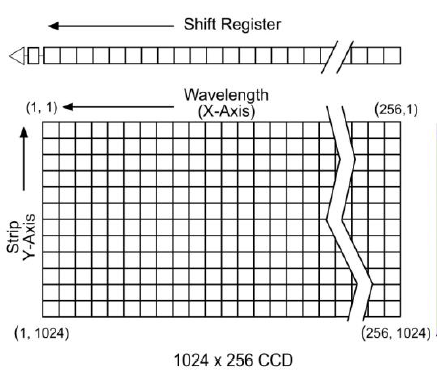
\includegraphics[width=0.5\textwidth]{pictures/1.PNG}
\caption{坐标轴定义。来自WinSpec User's Manual}
\end{figure}

\begin{itemize}
\item x1表示x轴选用的起始像素位置,x2表示x轴选用终止像素位置。y1,y2同理,表示y轴方向的像素选取。
\item x bin(binning),表示x轴每多少像素求和, y bin同理。为了增强信号,我们将y轴信号全部加起来,即 y bin 设置为 200。为了不降低分辨率,并没有对x轴信号进行部分求和,即 x bin 设置为1。
\end{itemize}
\textbf{WinSpec设置}: Acquisition>Experiment Setup
\begin{itemize}
\item Select Mode: Imaging Mode or Spectroscopy Mode
\item Clicking on \textbf{Full} loads the full size of the chip into the edit boxes.
\end{itemize}
\textbf{LightField设置}: Experiment Settings>Regions of Interest

\item 第三个子vi是示例vi: ExSubSetup.vi。This Sub VI sets up the skips, cleans, and shutter parameters. This should be changed to suit the camera you are using.由多个底层vi构成。
\begin{itemize}
\item 第一个底层vi:CameraCleans.vi。用来清除CCD芯片电荷的。
\\ \textbf{默认参数\footnote{这里默认参数指的是示例vi直接在后面板中设定好的参数}}:Number of Clears:1; Number of Strips Per Clear:50;  Continous Clears:0。
\\ \textbf{参数说明}:这部分参数说明要结合EMCDD说明书,参考其中Cleaning部分,这里摘抄如下。
\begin{itemize}
\item \emph{Number of Cleans} value is ususally set to one(1). These are additional clean cycles that can be required after a start exposure signal is received and the current clean cycle has finished. The maximum value for this entry depends on the camera.通常设为1。
\item \emph{Number of Strips per Clean} sets the number of rows that will be shifted 
and discarded per clean cycle. While a large number such as the number of rows in the array may result in the best cleaning of the array, the tradeoff is that there may be a significant delay between the receipt of a start exposure signal and the beginning of the actual exposure. This delay occurs because the current clean cycle must be completed before a start exposure signal received during the cycle will be implemented.Typically, the default setting is much smaller and in time critical experiments, the setting should be 1 or 2. 值越大清理的CCD行数越多,但是耗时也越多,需要用户权衡好。
\item \emph{Continuous Cleans} is available when the start of exposure is tied to an external trigger.This parameter is a flag that will allow clears to be performed "continuously" while running. This is the number o strips to clear before looking if an external trigger has arrived. This mode is usually used when collecting data with the camera in external trigger mode and the shutter disabled open.
\end{itemize}
\textbf{WinSpec设置}: Hardware Setup>Clean/Skips
\\ \textbf{LightField设置}: Experiment Settings>Sensor>Sensor Cleaning

\item 第二个底层vi:CameraShutter.vi。设置CCD的开和关。
\\\textbf{默认参数}:Shutter State:4;Shutter Compensation Time: Pre Open:0; Shutter Compensation Time: Post Open:0。
\\ \textbf{参数说明}:
\begin{itemize}
\item Shutter State设为4,表示CCD一直开着。
\item Shutter Compensation Time: Pre Open,只支持 Photometrics brand cameras 和 Acton InSpectrum camera,可以不连。
\item Shutter Compensation Time: Post Open的值必须设置,是CCD关闭的时间,单位是毫秒。
\end{itemize}
\textbf{WinSpec设置}:
\\ \textbf{LightField设置}: Experiment Settings>Shutter

\item 第三个底层vi:ToolKitIsError.vi。 检查SITK软件包是否有错误。
\end{itemize}

\item 第四个子vi是底层vi: CameraTrigger.vi。设置的是CCD信号触发模式。
\\ \textbf{默认参数}:Timing Mode:3(Strobed/Ext Sync);Trigger Edge:2。
\\ \textbf{参数说明}:
\begin{itemize}
\item Timing Mode:3表示选用的是外触发模式“Each exposure requires a trigger (Ext Sync, Strobed Mode)”;
\item Trigger Edge:2表示信号触发沿设定的是下降沿“Negative(falling) edge”。
\end{itemize}
\textbf{WinSpec设置}:
\\ \textbf{LightField设置}: Experiment Settings>Trigger>Readout Per Trigg

\item 第五个子vi是底层vi:CameraADCset.vi。 ADC,Analog to Digital Conversion,模拟信号转换为数字信号,模数转换。
\\ \textbf{默认参数}:ADC Speed:-2; ADC Gain:-1; Read Out port:-1; ADC offset:-1
\\ \textbf{参数说明}:
\begin{itemize}
\item ADC Speed: For Slowest ADC speed set this to -3; For Fastest ADC speed set this to -2; To use current ADC speed don't hook up or use -1 otherwise put speed in as KHz.
\item ADC Gain: To use current gain don't hook up or set to -1.
\item Read Out port: To use current readout port don't hook up or set to -1.
\item ADC offset: To use current offset don't hook up or set to -1.
\end{itemize}
\textbf{WinSpec设置}:
\\ \textbf{LightField设置}: Experiment Settings>Analog to Digital Conversion>Electron Multiplied

\item 第六个子vi是底层vi:CameraADCget.vi。获取当前模数转换的信息,示例vi中只输出了 ADC Speed 项。
\end{itemize}


(3)ExSetupExtSuperSyncro.vi:由一系列子vi构成,用来设置CCD的触发信号同步。
\begin{itemize}
\item 第一个子vi是示例vi: ExSubCheckCamPulser.vi。检查Camera和Pulser全局句柄是否创建。

\item 第二个子vi是示例vi: ExSubSetupCamPulserExtTrigSuperSync.vi。由一系列底层vi构成\footnote{注意:底层vi都是有详细说明文档的;底层vi中经常用到无符号长整型,但是用的时候可能用的有无符号长整型,虽然不会影响参数传递,但是在接口处有红点提示数据类型不是完全匹配}。
\begin{itemize}
\item 第一个底层vi是: CameraShutter.vi
\\ \textbf{与前面vi有重复,删除此处。}

\item 第二个底层vi是:CameraIntensMode.vi。设置光电倍增管的模式和强度。
\\ \textbf{参数}:Mode:2; Intensifier Gain: 20
\\ \textbf{参数说明}:
\begin{itemize}
\item Mode:2表示光电倍增管一直开着;
\item Intensifier Gain: 20表示增强值设为20。为什么是20不太清楚。
\end{itemize}
\textbf{WinSpec设置}:
\\ \textbf{LightField设置}: Experiment Settings>Analog to Digital Conversion>Electron Multiplied>EM Gain

\item 第三个底层vi是:CameraTrigger.vi
\\ \textbf{与前面vi有重复,删除此处。}


\item 第四个底层vi是:CameraCleans.vi
\\ \textbf{与前面vi有重复,删除此处。}

\item 第五个底层vi是:CameraSkips.vi
\\ \textbf{与前面vi有重复,删除此处。}

\item 第六个底层vi是:PulserExternalTrigger.vi。设置外触发模式以及相关参数。
\\ \textbf{参数}: Threshold:1; Slope:1; Coupling:1; Termination: 0
\\ \textbf{参数说明}: 
\begin{itemize}
\item Threshold:设置触发电压阈值,单位伏特(Volts)。
\item Slope:触发沿,0表示下降沿触发,表示上升沿触发。
\item Coupling:设置触发是交流(AC)触发还是直流(DC)触发,0表示ac,1表示dc。
\item Termination:设置阻抗,0表示50欧姆(Ohms),1表示高阻抗。
\end{itemize}
\textbf{Available only in Kinetics mode or DIF acquisition.}

\item 第七个底层vi是:PulserGateWidthDelay.vi。 This VI will set the gate width and delay values for repetitive pulsing in microseconds.
\\ \textbf{参数}: Gate Width: 0.1($\mu$s); Gate Delay: 0.0($\mu$s)
\\ \textbf{参数说明}:
\begin{itemize}
\item Gate Width: This value is the width of the gate pulse in microseconds.
\item Gate Delay: This value is the delay of the gate pulse in microseconds.
\end{itemize}

\item 第八个底层vi是:PulserOnChipAccum.vi。设置读取CCD芯片值前的曝光次数。
\\ \textbf{参数}: Accumulation:1
\\ \textbf{参数说明}:单脉冲测量关键,1表示曝光一次读取一次值,大于1表示曝光多次后读取一次值。

\item 第九个底层vi是:PulserSetVar.vi
\\ \textbf{默认参数}: Parameter ID:1002; Value:1601.0
\\ \textbf{参数说明}: Parameter ID,1002,表示Pulse Delay From;Value,1601.0表示 del from ext trig in, 而1602表示 del from t0 out.

\item 第十个底层vi是:PulserSetVar.vi
\\ \textbf{默认参数}: Parameter ID:1102; Value:0.0
\\ \textbf{参数说明}: Parameter ID,1102,表示Braket Pulse;Value,0.0表示 turn off braket pulse.
\end{itemize}
\end{itemize}


\section{PI-MAX3光谱采集LabVIEW程序解析}
CCD光谱采集LabVIEW程序是由示例程序 ExDataCollectPulserNframe.vi 改写过来的。这里详细说明下。
\begin{itemize}
\item 第一个子vi是示例vi: ExSubCheckCamPulser.vi。检查Camera和Pulser全局句柄是否创建。
\\ \textbf{初始化已经检查过了,这里删除?}

\item 第二个子vi是示例vi: ExSubInitCamPulser.vi。CCD初始化。由多个底层vi构成。
\begin{itemize}
\item 第一个底层vi是: CameraExperiment.vi。This function will allow the setup and running
of a basic data collection experiment. All advanced camera settings are set to good defaults.
\\ \textbf{参数}: Exposure(sec):0.0001(s,100$\mu$s); Number of Images: 200(\textbf{注:这里的严格表述应该为 Number of pulse})
\\ \textbf{默认参数}: Acquire/Focus Flag: 1; Number of Accumulations:1
\item 第二个底层vi是: PulserInit.vi。\textbf{什么是Pulser?}
\item 第三个底层vi是: CameraInitialzie.vi。初始化CCD,随时准备采集数据。
\end{itemize}

\item 第三个子vi是示例vi: ExSubCreateFileMultImage.vi由多个底层vi构成。
\\ \textbf{默认参数}:Number of Images:1。\textbf{和前面有重名需要进一步考察他们的功能。} 
\begin{itemize}
\item 第一个底层vi是: CameraGetDataDim.vi。This VI will return the X and Y dimension of one frame of data as defined in the camera.\textbf{不出意外,根据前面的设置,应该为1600*1,要测试下。}
\item 第二个底层vi是: ImageCreate.vi: This VI will create an image space to hold an image
of dimensions X and Y, number of frames and of the data type specified. A handle to this 
image is returned to provide access.
\\ \textbf{默认参数}: x dimension、y dimension:由前面vi获取得到;Data Type:4; Number of Frames: 1
\\ \textbf{参数说明}:
\begin{itemize}
\item X dimension: Number of data points in the X direction.
\item Y dimension: Number of data points in the Y direction.
\item Data Type: Type of binary representation of the data. 4=32-bit floating point
\item Number of Frames: Number of full frames of data X by Y in size.
\item Image Handle: A handle to image created is returned to provide access to the image. \textbf{Handle 到底是什么东西?}
\end{itemize}


\item 第三个底层vi是: FileOpen.vi。\textbf{并没有用到。}
\end{itemize}

\item 第四个子vi是示例vi:ExSubStartExpPulser.vi。由多个底层vi构成。
\begin{itemize}
\item 第一个底层vi是: PulserStart.vi
\item 第二个底层vi是: CameraStart.vi
\end{itemize}

\item 第五个子vi是示例vi: ExSubNframeColMultiImageFast.vi。由多个底层vi构成。
\\ \textbf{默认参数}:Number of Images:1。\textbf{和前面有重名需要进一步考察他们的功能。} 
\begin{itemize}
\item 第一个底层vi是: CameraCheckData.vi。This function will return the number of complete frames of data available to the calling function.
\item 第二个底层vi是: CameraGetData.vi。This VI will retrieve the data from the camera 
and store it in the data area of the data cluster parameter. The storage space for the
data must be pre-allocated by the caller. The dimensions to be allocated may be obtained
from the CameraGetDataDim VI.
\item 第三个底层vi是: ImageGetLineF32.vi。This VI will return a 1-dimensional line of data from an image in 32-bit Floating Point format. 
\\ \textbf{默认参数}: Y Position:1; Z Position:1
\\ \textbf{参数说明}:
\begin{itemize}
\item Data Handle: Handle to an image. This is obtained via the ImageCreate VI.
\item Z Position: This value is the 1-based position in the Z-axis of the frame of data from which the line of data is to be returned.
\item Y Position: This value is the 1-based position in the Y-axis of the line of data to be returned.
\end{itemize} 	
\end{itemize}

\item 第六个子vi是底层vi: ImageDestroy.vi

\item 第七个子vi是示例vi: ExSubStopCamPulser.vi。
\begin{itemize}
\item 第一个底层vi是: CameraStop.vi
\item 第二个底层vi是: PulserStop.vi
\end{itemize}
\end{itemize}



\chapter{R}

\section{Install R on Mac}
直接去官网下载安装即可, \url{https://cran.r-project.org/bin/macosx/}。
然后去下载免费的代码编辑器 RStudio。

\section{常用的packages}

\subsection{ggplot2}
\subsection{data.table}
\subsection{tidyverse}
\subsection{magritter}
\subsection{patchwork}
\subsection{fs}
\subsection{rvest}
\subsection{purr}
\subsection{drake}
\begin{itemize}
\item drake$\_$plan: create a workflow data frame
\item make: build your project
\item vis$\_$drake$\_$graph: show an interactive visual network representation of your workflow
\item drake$\_$history: show what you built, when you built in, and the function arguments you used
\item loadd: load one or more built targets into your R session
\item readd: read and return a built target
\item outdated: see which targets will be built in the next make
\item deps: check the dependencies of a command or function
\item failed: list the targets that failed to build in the last make
\item diagnose: return the full context of a build, including errors, warnings, and messages
\end{itemize}

\subsection{janitor}
- comment style
\subsection{httr}
Use GET function to connect with website and get data from it.
\subsection{V8}

\section{小贴士}
\begin{itemize}
\item never use these two commands in the head of R script
\begin{itemize}
\item first (instead use here::here())
\begin{lstlisting}[language=R]
setwd("**/**/**")
\end{lstlisting}
\item second 
\begin{lstlisting}[language=R]
rm(list = ls())
\end{lstlisting}
Don't try to change the .Rprofile and affect the data
\end{itemize}

\item check the loaded packages
\begin{lstlisting}[language=R]
(.packages())
\end{lstlisting}

\item set the working directory
\begin{lstlisting}[language=R]
setwd()
\end{lstlisting}
I custom the short key in R with \emph{Cmd+Shift+H}.

\item tidy code's formatation
Here I just introduce the tidy method in RStudio.
1. select the region, e.g. \emph{Cmd + A}
2. print shortcuting \emph{Cmd + Shift + A} to format the code or run **style active file** in addin

\item get file's path
\begin{lstlisting}[language=R]
full_path <- normalizePath(file_eg)
dir_name<-dirname()
file_name<-basename()
\end{lstlisting}

\item insert and run R chunck in Rmarkdown
insert:\emph{Cmd+Opt+i}
run: \emph{Cmd+Shift+enter}

\end{itemize}

\chapter{Julia}

\section{Install Julia on Mac}










